\documentclass[twoside]{book}

% Packages required by doxygen
\usepackage{fixltx2e}
\usepackage{calc}
\usepackage{doxygen}
\usepackage[export]{adjustbox} % also loads graphicx
\usepackage{graphicx}
\usepackage[utf8]{inputenc}
\usepackage{makeidx}
\usepackage{multicol}
\usepackage{multirow}
\PassOptionsToPackage{warn}{textcomp}
\usepackage{textcomp}
\usepackage[nointegrals]{wasysym}
\usepackage[table]{xcolor}

% Font selection
\usepackage[T1]{fontenc}
\usepackage[scaled=.90]{helvet}
\usepackage{courier}
\usepackage{amssymb}
\usepackage{sectsty}
\renewcommand{\familydefault}{\sfdefault}
\allsectionsfont{%
  \fontseries{bc}\selectfont%
  \color{darkgray}%
}
\renewcommand{\DoxyLabelFont}{%
  \fontseries{bc}\selectfont%
  \color{darkgray}%
}
\newcommand{\+}{\discretionary{\mbox{\scriptsize$\hookleftarrow$}}{}{}}

% Page & text layout
\usepackage{geometry}
\geometry{%
  a4paper,%
  top=2.5cm,%
  bottom=2.5cm,%
  left=2.5cm,%
  right=2.5cm%
}
\tolerance=750
\hfuzz=15pt
\hbadness=750
\setlength{\emergencystretch}{15pt}
\setlength{\parindent}{0cm}
\setlength{\parskip}{3ex plus 2ex minus 2ex}
\makeatletter
\renewcommand{\paragraph}{%
  \@startsection{paragraph}{4}{0ex}{-1.0ex}{1.0ex}{%
    \normalfont\normalsize\bfseries\SS@parafont%
  }%
}
\renewcommand{\subparagraph}{%
  \@startsection{subparagraph}{5}{0ex}{-1.0ex}{1.0ex}{%
    \normalfont\normalsize\bfseries\SS@subparafont%
  }%
}
\makeatother

% Headers & footers
\usepackage{fancyhdr}
\pagestyle{fancyplain}
\fancyhead[LE]{\fancyplain{}{\bfseries\thepage}}
\fancyhead[CE]{\fancyplain{}{}}
\fancyhead[RE]{\fancyplain{}{\bfseries\leftmark}}
\fancyhead[LO]{\fancyplain{}{\bfseries\rightmark}}
\fancyhead[CO]{\fancyplain{}{}}
\fancyhead[RO]{\fancyplain{}{\bfseries\thepage}}
\fancyfoot[LE]{\fancyplain{}{}}
\fancyfoot[CE]{\fancyplain{}{}}
\fancyfoot[RE]{\fancyplain{}{\bfseries\scriptsize Generated by Doxygen }}
\fancyfoot[LO]{\fancyplain{}{\bfseries\scriptsize Generated by Doxygen }}
\fancyfoot[CO]{\fancyplain{}{}}
\fancyfoot[RO]{\fancyplain{}{}}
\renewcommand{\footrulewidth}{0.4pt}
\renewcommand{\chaptermark}[1]{%
  \markboth{#1}{}%
}
\renewcommand{\sectionmark}[1]{%
  \markright{\thesection\ #1}%
}

% Indices & bibliography
\usepackage{natbib}
\usepackage[titles]{tocloft}
\setcounter{tocdepth}{3}
\setcounter{secnumdepth}{5}
\makeindex

% Hyperlinks (required, but should be loaded last)
\usepackage{ifpdf}
\ifpdf
  \usepackage[pdftex,pagebackref=true]{hyperref}
\else
  \usepackage[ps2pdf,pagebackref=true]{hyperref}
\fi
\hypersetup{%
  colorlinks=true,%
  linkcolor=blue,%
  citecolor=blue,%
  unicode%
}

% Custom commands
\newcommand{\clearemptydoublepage}{%
  \newpage{\pagestyle{empty}\cleardoublepage}%
}

\usepackage{caption}
\captionsetup{labelsep=space,justification=centering,font={bf},singlelinecheck=off,skip=4pt,position=top}

%===== C O N T E N T S =====

\begin{document}

% Titlepage & ToC
\hypersetup{pageanchor=false,
             bookmarksnumbered=true,
             pdfencoding=unicode
            }
\pagenumbering{alph}
\begin{titlepage}
\vspace*{7cm}
\begin{center}%
{\Large My Project }\\
\vspace*{1cm}
{\large Generated by Doxygen 1.8.13}\\
\end{center}
\end{titlepage}
\clearemptydoublepage
\pagenumbering{roman}
\tableofcontents
\clearemptydoublepage
\pagenumbering{arabic}
\hypersetup{pageanchor=true}

%--- Begin generated contents ---
\chapter{Hierarchical Index}
\section{Class Hierarchy}
This inheritance list is sorted roughly, but not completely, alphabetically\+:\begin{DoxyCompactList}
\item \contentsline{section}{C\+Calibration}{\pageref{classCCalibration}}{}
\item \contentsline{section}{C\+Communicate}{\pageref{classCCommunicate}}{}
\item \contentsline{section}{C\+Configuration}{\pageref{classCConfiguration}}{}
\item \contentsline{section}{C\+Event}{\pageref{classCEvent}}{}
\item \contentsline{section}{C\+Move}{\pageref{classCMove}}{}
\item \contentsline{section}{C\+Robot\+Context}{\pageref{classCRobotContext}}{}
\item \contentsline{section}{C\+Servo\+Instruction}{\pageref{classCServoInstruction}}{}
\item \contentsline{section}{C\+State\+Publisher}{\pageref{classCStatePublisher}}{}
\item \contentsline{section}{I\+Execute\+Command}{\pageref{classIExecuteCommand}}{}
\begin{DoxyCompactList}
\item \contentsline{section}{C\+Command\+A\+L5D}{\pageref{classCCommandAL5D}}{}
\end{DoxyCompactList}
\item \contentsline{section}{I\+Robot\+States}{\pageref{classIRobotStates}}{}
\begin{DoxyCompactList}
\item \contentsline{section}{C\+Calibrate\+State}{\pageref{classCCalibrateState}}{}
\item \contentsline{section}{C\+Idle\+State}{\pageref{classCIdleState}}{}
\item \contentsline{section}{C\+Move\+State}{\pageref{classCMoveState}}{}
\item \contentsline{section}{C\+Stop\+State}{\pageref{classCStopState}}{}
\end{DoxyCompactList}
\end{DoxyCompactList}

\chapter{Class Index}
\section{Class List}
Here are the classes, structs, unions and interfaces with brief descriptions\+:\begin{DoxyCompactList}
\item\contentsline{section}{\hyperlink{classCCalibrateState}{C\+Calibrate\+State} }{\pageref{classCCalibrateState}}{}
\item\contentsline{section}{\hyperlink{classCCalibration}{C\+Calibration} }{\pageref{classCCalibration}}{}
\item\contentsline{section}{\hyperlink{classCCommandAL5D}{C\+Command\+A\+L5D} }{\pageref{classCCommandAL5D}}{}
\item\contentsline{section}{\hyperlink{classCCommunicate}{C\+Communicate} }{\pageref{classCCommunicate}}{}
\item\contentsline{section}{\hyperlink{classCConfiguration}{C\+Configuration} }{\pageref{classCConfiguration}}{}
\item\contentsline{section}{\hyperlink{classCEvent}{C\+Event} }{\pageref{classCEvent}}{}
\item\contentsline{section}{\hyperlink{classCIdleState}{C\+Idle\+State} }{\pageref{classCIdleState}}{}
\item\contentsline{section}{\hyperlink{classCMove}{C\+Move} }{\pageref{classCMove}}{}
\item\contentsline{section}{\hyperlink{classCMoveState}{C\+Move\+State} }{\pageref{classCMoveState}}{}
\item\contentsline{section}{\hyperlink{classCRobotContext}{C\+Robot\+Context} }{\pageref{classCRobotContext}}{}
\item\contentsline{section}{\hyperlink{classCServoInstruction}{C\+Servo\+Instruction} }{\pageref{classCServoInstruction}}{}
\item\contentsline{section}{\hyperlink{classCStatePublisher}{C\+State\+Publisher} }{\pageref{classCStatePublisher}}{}
\item\contentsline{section}{\hyperlink{classCStopState}{C\+Stop\+State} }{\pageref{classCStopState}}{}
\item\contentsline{section}{\hyperlink{classIExecuteCommand}{I\+Execute\+Command} }{\pageref{classIExecuteCommand}}{}
\item\contentsline{section}{\hyperlink{classIRobotStates}{I\+Robot\+States} }{\pageref{classIRobotStates}}{}
\end{DoxyCompactList}

\chapter{File Index}
\section{File List}
Here is a list of all documented files with brief descriptions\+:\begin{DoxyCompactList}
\item\contentsline{section}{\hyperlink{CEvent_8h}{C\+Event.\+h} \\*The \hyperlink{classCEvent}{C\+Event} class is used as an event for the State machine, it holds instructions for servos and an eventtype to be used in the state machine }{\pageref{CEvent_8h}}{}
\item\contentsline{section}{\hyperlink{CRobotContext_8h}{C\+Robot\+Context.\+h} \\*The \hyperlink{classCRobotContext}{C\+Robot\+Context} is the context for the state machine which controlls the robot arm through its states of moving, idling, calibrating, and stopping. It also holds a nodehandle with which it subscribes to ros topics on which instructions get published }{\pageref{CRobotContext_8h}}{}
\item\contentsline{section}{\hyperlink{CServoInstruction_8h}{C\+Servo\+Instruction.\+h} \\*C\+Servoinstruction is a class that holds the instructions for a specfic servo within the robotarm }{\pageref{CServoInstruction_8h}}{}
\item\contentsline{section}{\hyperlink{CStatePublisher_8h}{C\+State\+Publisher.\+h} \\*\hyperlink{classCStatePublisher}{C\+State\+Publisher} is a singleton class that can be used to publish a state on the /\+Robot\+Arm\+Controller/\+State ros topic }{\pageref{CStatePublisher_8h}}{}
\item\contentsline{section}{\hyperlink{CStates_8h}{C\+States.\+h} \\*In this file are the various states which the Robot\+Arm\+Controller\textquotesingle{}s state machine can be in }{\pageref{CStates_8h}}{}
\item\contentsline{section}{\hyperlink{IRobotStates_8h}{I\+Robot\+States.\+h} \\*The interface for the various classes in the state machine }{\pageref{IRobotStates_8h}}{}
\item\contentsline{section}{Robot\+High\+Level/\hyperlink{CCalibration_8cpp}{C\+Calibration.\+cpp} }{\pageref{CCalibration_8cpp}}{}
\item\contentsline{section}{Robot\+High\+Level/\hyperlink{CCalibration_8h}{C\+Calibration.\+h} \\*The Calibration class is responsible for handling calibrations for the servo boundries }{\pageref{CCalibration_8h}}{}
\item\contentsline{section}{Robot\+High\+Level/\hyperlink{CConfiguration_8cpp}{C\+Configuration.\+cpp} }{\pageref{CConfiguration_8cpp}}{}
\item\contentsline{section}{Robot\+High\+Level/\hyperlink{CConfiguration_8h}{C\+Configuration.\+h} \\*The configuration class holds the calibrated values for every servo }{\pageref{CConfiguration_8h}}{}
\item\contentsline{section}{Robot\+High\+Level/\hyperlink{CMove_8cpp}{C\+Move.\+cpp} }{\pageref{CMove_8cpp}}{}
\item\contentsline{section}{Robot\+High\+Level/\hyperlink{CMove_8h}{C\+Move.\+h} \\*The \hyperlink{classCMove}{C\+Move} class offers functions to calculate degrees to P\+WM and to then send a command to the robotarm that will make it move }{\pageref{CMove_8h}}{}
\item\contentsline{section}{Robot\+Low\+Level/\hyperlink{CCommandAL5D_8cpp}{C\+Command\+A\+L5\+D.\+cpp} }{\pageref{CCommandAL5D_8cpp}}{}
\item\contentsline{section}{Robot\+Low\+Level/\hyperlink{CCommandAL5D_8h}{C\+Command\+A\+L5\+D.\+h} \\*The Command\+A\+L5D class is a realistation of the \hyperlink{classIExecuteCommand}{I\+Execute\+Command}. It is reponsible for commanding the A\+L5D robotarm and is used by higher level drivers }{\pageref{CCommandAL5D_8h}}{}
\item\contentsline{section}{Robot\+Low\+Level/\hyperlink{CCommunicate_8cpp}{C\+Communicate.\+cpp} }{\pageref{CCommunicate_8cpp}}{}
\item\contentsline{section}{Robot\+Low\+Level/\hyperlink{CCommunicate_8h}{C\+Communicate.\+h} \\*The communicate class makes use of boost asio messaging to write messages to the robotarm through the serial output }{\pageref{CCommunicate_8h}}{}
\item\contentsline{section}{Robot\+Low\+Level/\hyperlink{IExecuteCommand_8h}{I\+Execute\+Command.\+h} \\*The Execute\+Command interfaces gives higher level drivers the ability to send instructions to the robotarm }{\pageref{IExecuteCommand_8h}}{}
\end{DoxyCompactList}

\chapter{Class Documentation}
\hypertarget{classCCalibrateState}{}\section{C\+Calibrate\+State Class Reference}
\label{classCCalibrateState}\index{C\+Calibrate\+State@{C\+Calibrate\+State}}


Inheritance diagram for C\+Calibrate\+State\+:\nopagebreak
\begin{figure}[H]
\begin{center}
\leavevmode
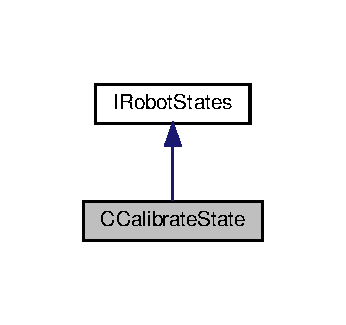
\includegraphics[width=166pt]{classCCalibrateState__inherit__graph}
\end{center}
\end{figure}


Collaboration diagram for C\+Calibrate\+State\+:\nopagebreak
\begin{figure}[H]
\begin{center}
\leavevmode
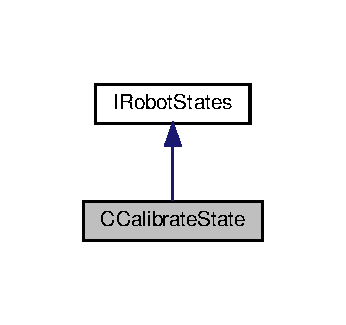
\includegraphics[width=166pt]{classCCalibrateState__coll__graph}
\end{center}
\end{figure}
\subsection*{Public Member Functions}
\begin{DoxyCompactItemize}
\item 
\hyperlink{classCCalibrateState_aac8ef64d3e1d849d6e0dee9d219585b6}{C\+Calibrate\+State} (\hyperlink{classCEvent}{C\+Event} \&r\+Event, std\+::shared\+\_\+ptr$<$ \hyperlink{classCConfiguration}{C\+Configuration} $>$ sp\+Configuration)
\begin{DoxyCompactList}\small\item\em The state a Robot\+Arm\+Controller is in while it is calibrating movement in this state will be used in the configuration class as a calibration. \end{DoxyCompactList}\item 
void \hyperlink{classCCalibrateState_a361368643bad182ed1a78ee1d1a820e5}{Entry} ()
\begin{DoxyCompactList}\small\item\em the entry action which will be executed for the various states when the context enters that state. \end{DoxyCompactList}\item 
void \hyperlink{classCCalibrateState_a2b2ad369ae655704fadcffb0a4b9fca2}{Do} ()
\begin{DoxyCompactList}\small\item\em The do activity which will be executed after the entry action for the various states when the context enters that state. \end{DoxyCompactList}\item 
void \hyperlink{classCCalibrateState_a0bdb13da2af72f1e8e814a365f8d765a}{Exit} ()
\begin{DoxyCompactList}\small\item\em The exit action which will executed when the context transitions off of the state. \end{DoxyCompactList}\item 
void \hyperlink{classCCalibrateState_af24b30b6357a7b48f1157afdc0662984}{Handle\+Event} (\hyperlink{classCEvent}{C\+Event} \&r\+Event, \hyperlink{classCRobotContext}{C\+Robot\+Context} \&r\+Context)
\begin{DoxyCompactList}\small\item\em The Handle\+Event function defines how the context will react to the next event, this depends on the state it is currently in. \end{DoxyCompactList}\end{DoxyCompactItemize}


\subsection{Constructor \& Destructor Documentation}
\mbox{\Hypertarget{classCCalibrateState_aac8ef64d3e1d849d6e0dee9d219585b6}\label{classCCalibrateState_aac8ef64d3e1d849d6e0dee9d219585b6}} 
\index{C\+Calibrate\+State@{C\+Calibrate\+State}!C\+Calibrate\+State@{C\+Calibrate\+State}}
\index{C\+Calibrate\+State@{C\+Calibrate\+State}!C\+Calibrate\+State@{C\+Calibrate\+State}}
\subsubsection{\texorpdfstring{C\+Calibrate\+State()}{CCalibrateState()}}
{\footnotesize\ttfamily C\+Calibrate\+State\+::\+C\+Calibrate\+State (\begin{DoxyParamCaption}\item[{\hyperlink{classCEvent}{C\+Event} \&}]{r\+Event,  }\item[{std\+::shared\+\_\+ptr$<$ \hyperlink{classCConfiguration}{C\+Configuration} $>$}]{sp\+Configuration }\end{DoxyParamCaption})}



The state a Robot\+Arm\+Controller is in while it is calibrating movement in this state will be used in the configuration class as a calibration. 


\begin{DoxyParams}{Parameters}
{\em r\+Event} & The event that triggered this state \\
\hline
{\em sp\+Configuration} & the Configuration with the calibrated values for the robotarm, this will be passed when the handle\+Event function is called onto other states. \\
\hline
\end{DoxyParams}


\subsection{Member Function Documentation}
\mbox{\Hypertarget{classCCalibrateState_a2b2ad369ae655704fadcffb0a4b9fca2}\label{classCCalibrateState_a2b2ad369ae655704fadcffb0a4b9fca2}} 
\index{C\+Calibrate\+State@{C\+Calibrate\+State}!Do@{Do}}
\index{Do@{Do}!C\+Calibrate\+State@{C\+Calibrate\+State}}
\subsubsection{\texorpdfstring{Do()}{Do()}}
{\footnotesize\ttfamily void C\+Calibrate\+State\+::\+Do (\begin{DoxyParamCaption}{ }\end{DoxyParamCaption})\hspace{0.3cm}{\ttfamily [virtual]}}



The do activity which will be executed after the entry action for the various states when the context enters that state. 



Implements \hyperlink{classIRobotStates_aa681381e72738a2870c3f13f552a2e93}{I\+Robot\+States}.

\mbox{\Hypertarget{classCCalibrateState_a361368643bad182ed1a78ee1d1a820e5}\label{classCCalibrateState_a361368643bad182ed1a78ee1d1a820e5}} 
\index{C\+Calibrate\+State@{C\+Calibrate\+State}!Entry@{Entry}}
\index{Entry@{Entry}!C\+Calibrate\+State@{C\+Calibrate\+State}}
\subsubsection{\texorpdfstring{Entry()}{Entry()}}
{\footnotesize\ttfamily void C\+Calibrate\+State\+::\+Entry (\begin{DoxyParamCaption}{ }\end{DoxyParamCaption})\hspace{0.3cm}{\ttfamily [virtual]}}



the entry action which will be executed for the various states when the context enters that state. 



Implements \hyperlink{classIRobotStates_af43ddb52f5100b42c3d11b71fb1f10dd}{I\+Robot\+States}.

\mbox{\Hypertarget{classCCalibrateState_a0bdb13da2af72f1e8e814a365f8d765a}\label{classCCalibrateState_a0bdb13da2af72f1e8e814a365f8d765a}} 
\index{C\+Calibrate\+State@{C\+Calibrate\+State}!Exit@{Exit}}
\index{Exit@{Exit}!C\+Calibrate\+State@{C\+Calibrate\+State}}
\subsubsection{\texorpdfstring{Exit()}{Exit()}}
{\footnotesize\ttfamily void C\+Calibrate\+State\+::\+Exit (\begin{DoxyParamCaption}{ }\end{DoxyParamCaption})\hspace{0.3cm}{\ttfamily [virtual]}}



The exit action which will executed when the context transitions off of the state. 



Implements \hyperlink{classIRobotStates_a099417875e67f047ca38e08890491529}{I\+Robot\+States}.

\mbox{\Hypertarget{classCCalibrateState_af24b30b6357a7b48f1157afdc0662984}\label{classCCalibrateState_af24b30b6357a7b48f1157afdc0662984}} 
\index{C\+Calibrate\+State@{C\+Calibrate\+State}!Handle\+Event@{Handle\+Event}}
\index{Handle\+Event@{Handle\+Event}!C\+Calibrate\+State@{C\+Calibrate\+State}}
\subsubsection{\texorpdfstring{Handle\+Event()}{HandleEvent()}}
{\footnotesize\ttfamily void C\+Calibrate\+State\+::\+Handle\+Event (\begin{DoxyParamCaption}\item[{\hyperlink{classCEvent}{C\+Event} \&}]{r\+Event,  }\item[{\hyperlink{classCRobotContext}{C\+Robot\+Context} \&}]{r\+Context }\end{DoxyParamCaption})\hspace{0.3cm}{\ttfamily [virtual]}}



The Handle\+Event function defines how the context will react to the next event, this depends on the state it is currently in. 


\begin{DoxyParams}{Parameters}
{\em r\+Event} & The next event to be handle by the state machine \\
\hline
{\em r\+Context} & The context which will go through a state because of the incoming event. \\
\hline
\end{DoxyParams}


Implements \hyperlink{classIRobotStates_a0b6c28a3deed04f93371a9395022f1ed}{I\+Robot\+States}.



The documentation for this class was generated from the following files\+:\begin{DoxyCompactItemize}
\item 
\hyperlink{CStates_8h}{C\+States.\+h}\item 
C\+States.\+cpp\end{DoxyCompactItemize}

\hypertarget{classCCalibration}{}\section{C\+Calibration Class Reference}
\label{classCCalibration}\index{C\+Calibration@{C\+Calibration}}
\subsection*{Public Member Functions}
\begin{DoxyCompactItemize}
\item 
\mbox{\Hypertarget{classCCalibration_a75081bf25db698d8aad2ab0398bc3ea0}\label{classCCalibration_a75081bf25db698d8aad2ab0398bc3ea0}} 
{\bfseries C\+Calibration} (std\+::shared\+\_\+ptr$<$ \hyperlink{classCConfiguration}{C\+Configuration} $>$ sp\+Configuration)
\item 
void \hyperlink{classCCalibration_a7174f917aab0eec5fbfc5f9f7ea2dcfb}{Execute} (e\+Command e\+Command, std\+::vector$<$ std\+::shared\+\_\+ptr$<$ \hyperlink{classCServoInstruction}{C\+Servo\+Instruction} $>$$>$ r\+Servo\+Intructions)
\begin{DoxyCompactList}\small\item\em Executes a list of servoinstructions. \end{DoxyCompactList}\end{DoxyCompactItemize}


\subsection{Member Function Documentation}
\mbox{\Hypertarget{classCCalibration_a7174f917aab0eec5fbfc5f9f7ea2dcfb}\label{classCCalibration_a7174f917aab0eec5fbfc5f9f7ea2dcfb}} 
\index{C\+Calibration@{C\+Calibration}!Execute@{Execute}}
\index{Execute@{Execute}!C\+Calibration@{C\+Calibration}}
\subsubsection{\texorpdfstring{Execute()}{Execute()}}
{\footnotesize\ttfamily void C\+Calibration\+::\+Execute (\begin{DoxyParamCaption}\item[{e\+Command}]{e\+Command,  }\item[{std\+::vector$<$ std\+::shared\+\_\+ptr$<$ \hyperlink{classCServoInstruction}{C\+Servo\+Instruction} $>$$>$}]{r\+Servo\+Intructions }\end{DoxyParamCaption})}



Executes a list of servoinstructions. 


\begin{DoxyParams}{Parameters}
{\em e\+Command} & the type of command(usually a C\+A\+L\+I\+B\+R\+A\+T\+E\+\_\+\+C\+O\+M\+M\+A\+N\+D when used within this class) \\
\hline
{\em r\+Servo\+Intructions} & the servoinstructions to have the robotarm execute \\
\hline
\end{DoxyParams}


The documentation for this class was generated from the following files\+:\begin{DoxyCompactItemize}
\item 
Robot\+High\+Level/\hyperlink{CCalibration_8h}{C\+Calibration.\+h}\item 
Robot\+High\+Level/\hyperlink{CCalibration_8cpp}{C\+Calibration.\+cpp}\end{DoxyCompactItemize}

\hypertarget{classCCommandAL5D}{}\section{C\+Command\+A\+L5D Class Reference}
\label{classCCommandAL5D}\index{C\+Command\+A\+L5D@{C\+Command\+A\+L5D}}


Inheritance diagram for C\+Command\+A\+L5D\+:\nopagebreak
\begin{figure}[H]
\begin{center}
\leavevmode
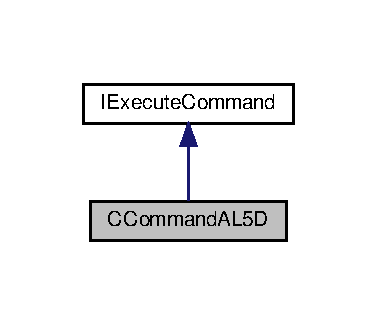
\includegraphics[width=181pt]{classCCommandAL5D__inherit__graph}
\end{center}
\end{figure}


Collaboration diagram for C\+Command\+A\+L5D\+:\nopagebreak
\begin{figure}[H]
\begin{center}
\leavevmode
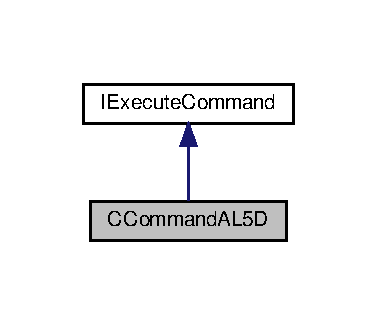
\includegraphics[width=181pt]{classCCommandAL5D__coll__graph}
\end{center}
\end{figure}
\subsection*{Public Member Functions}
\begin{DoxyCompactItemize}
\item 
void \hyperlink{classCCommandAL5D_a3cd260bd7bf8b4aa72dacc1d1ef2d38b}{Stop} () override
\begin{DoxyCompactList}\small\item\em This function will be called to stop communication to the robotarm. \end{DoxyCompactList}\item 
void \hyperlink{classCCommandAL5D_a308c945d4ed4009c85158a72e5db1bd5}{Write} (const std\+::string \&r\+Message) override
\begin{DoxyCompactList}\small\item\em The write function is called to write a string message to the robotarm. \end{DoxyCompactList}\item 
void \hyperlink{classCCommandAL5D_ae8b75aec364029b7cb65959325b6b9f7}{Append\+Instruction} (e\+Command e\+Command, int8\+\_\+t servo, int64\+\_\+t position, int64\+\_\+t speed, int64\+\_\+t duration) override
\begin{DoxyCompactList}\small\item\em the Append\+Instruction function adds an instruction to the list of instructions to send to the robotarm \end{DoxyCompactList}\item 
void \hyperlink{classCCommandAL5D_a46f133aa4b243af59e02f2cc23b12aa3}{Clear\+Lists} () override
\begin{DoxyCompactList}\small\item\em The clearlists function clears all the previously appended instructions. \end{DoxyCompactList}\item 
void \hyperlink{classCCommandAL5D_ac225e1c103a802a9276f201c94281ae2}{Execute} () override
\begin{DoxyCompactList}\small\item\em The execute function writes the stored instructions as a message to the robotarm. \end{DoxyCompactList}\end{DoxyCompactItemize}


\subsection{Member Function Documentation}
\mbox{\Hypertarget{classCCommandAL5D_ae8b75aec364029b7cb65959325b6b9f7}\label{classCCommandAL5D_ae8b75aec364029b7cb65959325b6b9f7}} 
\index{C\+Command\+A\+L5D@{C\+Command\+A\+L5D}!Append\+Instruction@{Append\+Instruction}}
\index{Append\+Instruction@{Append\+Instruction}!C\+Command\+A\+L5D@{C\+Command\+A\+L5D}}
\subsubsection{\texorpdfstring{Append\+Instruction()}{AppendInstruction()}}
{\footnotesize\ttfamily void C\+Command\+A\+L5\+D\+::\+Append\+Instruction (\begin{DoxyParamCaption}\item[{e\+Command}]{e\+Command,  }\item[{int8\+\_\+t}]{servo,  }\item[{int64\+\_\+t}]{position,  }\item[{int64\+\_\+t}]{speed,  }\item[{int64\+\_\+t}]{duration }\end{DoxyParamCaption})\hspace{0.3cm}{\ttfamily [override]}, {\ttfamily [virtual]}}



the Append\+Instruction function adds an instruction to the list of instructions to send to the robotarm 


\begin{DoxyParams}{Parameters}
{\em e\+Command} & the type of command to send to the servo \\
\hline
{\em servo} & the servo to control \\
\hline
{\em position} & the position to which the servo has to travel in P\+WM \\
\hline
{\em speed} & the maximum speed of the movement \\
\hline
{\em duration} & the duration of the movement \\
\hline
\end{DoxyParams}


Implements \hyperlink{classIExecuteCommand_a0f05e1cf668740504e36de8f662c0864}{I\+Execute\+Command}.

\mbox{\Hypertarget{classCCommandAL5D_a46f133aa4b243af59e02f2cc23b12aa3}\label{classCCommandAL5D_a46f133aa4b243af59e02f2cc23b12aa3}} 
\index{C\+Command\+A\+L5D@{C\+Command\+A\+L5D}!Clear\+Lists@{Clear\+Lists}}
\index{Clear\+Lists@{Clear\+Lists}!C\+Command\+A\+L5D@{C\+Command\+A\+L5D}}
\subsubsection{\texorpdfstring{Clear\+Lists()}{ClearLists()}}
{\footnotesize\ttfamily void C\+Command\+A\+L5\+D\+::\+Clear\+Lists (\begin{DoxyParamCaption}{ }\end{DoxyParamCaption})\hspace{0.3cm}{\ttfamily [override]}, {\ttfamily [virtual]}}



The clearlists function clears all the previously appended instructions. 



Implements \hyperlink{classIExecuteCommand_a34d2dc6186873e0f6f039fd4b41e414a}{I\+Execute\+Command}.

\mbox{\Hypertarget{classCCommandAL5D_ac225e1c103a802a9276f201c94281ae2}\label{classCCommandAL5D_ac225e1c103a802a9276f201c94281ae2}} 
\index{C\+Command\+A\+L5D@{C\+Command\+A\+L5D}!Execute@{Execute}}
\index{Execute@{Execute}!C\+Command\+A\+L5D@{C\+Command\+A\+L5D}}
\subsubsection{\texorpdfstring{Execute()}{Execute()}}
{\footnotesize\ttfamily void C\+Command\+A\+L5\+D\+::\+Execute (\begin{DoxyParamCaption}{ }\end{DoxyParamCaption})\hspace{0.3cm}{\ttfamily [override]}, {\ttfamily [virtual]}}



The execute function writes the stored instructions as a message to the robotarm. 



Implements \hyperlink{classIExecuteCommand_a8180d6931ffae55f04f9984d45a9c99f}{I\+Execute\+Command}.

\mbox{\Hypertarget{classCCommandAL5D_a3cd260bd7bf8b4aa72dacc1d1ef2d38b}\label{classCCommandAL5D_a3cd260bd7bf8b4aa72dacc1d1ef2d38b}} 
\index{C\+Command\+A\+L5D@{C\+Command\+A\+L5D}!Stop@{Stop}}
\index{Stop@{Stop}!C\+Command\+A\+L5D@{C\+Command\+A\+L5D}}
\subsubsection{\texorpdfstring{Stop()}{Stop()}}
{\footnotesize\ttfamily void C\+Command\+A\+L5\+D\+::\+Stop (\begin{DoxyParamCaption}{ }\end{DoxyParamCaption})\hspace{0.3cm}{\ttfamily [override]}, {\ttfamily [virtual]}}



This function will be called to stop communication to the robotarm. 



Implements \hyperlink{classIExecuteCommand_a9aaabaf7284c9d295c6e2fdfc1445ca4}{I\+Execute\+Command}.

\mbox{\Hypertarget{classCCommandAL5D_a308c945d4ed4009c85158a72e5db1bd5}\label{classCCommandAL5D_a308c945d4ed4009c85158a72e5db1bd5}} 
\index{C\+Command\+A\+L5D@{C\+Command\+A\+L5D}!Write@{Write}}
\index{Write@{Write}!C\+Command\+A\+L5D@{C\+Command\+A\+L5D}}
\subsubsection{\texorpdfstring{Write()}{Write()}}
{\footnotesize\ttfamily void C\+Command\+A\+L5\+D\+::\+Write (\begin{DoxyParamCaption}\item[{const std\+::string \&}]{r\+Message }\end{DoxyParamCaption})\hspace{0.3cm}{\ttfamily [override]}, {\ttfamily [virtual]}}



The write function is called to write a string message to the robotarm. 


\begin{DoxyParams}{Parameters}
{\em r\+Message} & the string which will be sent to the robotarm \\
\hline
\end{DoxyParams}


Implements \hyperlink{classIExecuteCommand_a266571b3fc97e79be6e00b0df4c5a4ac}{I\+Execute\+Command}.



The documentation for this class was generated from the following files\+:\begin{DoxyCompactItemize}
\item 
Robot\+Low\+Level/\hyperlink{CCommandAL5D_8h}{C\+Command\+A\+L5\+D.\+h}\item 
Robot\+Low\+Level/\hyperlink{CCommandAL5D_8cpp}{C\+Command\+A\+L5\+D.\+cpp}\end{DoxyCompactItemize}

\hypertarget{classCCommunicate}{}\section{C\+Communicate Class Reference}
\label{classCCommunicate}\index{C\+Communicate@{C\+Communicate}}
\subsection*{Public Member Functions}
\begin{DoxyCompactItemize}
\item 
bool \hyperlink{classCCommunicate_ab410d966213135d9d5c9ede493c5c5d8}{Init} ()
\begin{DoxyCompactList}\small\item\em Initialises the serial communication. \end{DoxyCompactList}\item 
bool \hyperlink{classCCommunicate_ab1eefe862756c613c4d006902badfffa}{Close} ()
\begin{DoxyCompactList}\small\item\em Closes the serial port if it was open. \end{DoxyCompactList}\item 
bool \hyperlink{classCCommunicate_a322f1dc7ffdd18be70e6e6aa9eca3613}{Write\+Serial} (const std\+::string \&r\+Message)
\begin{DoxyCompactList}\small\item\em Writes a string message to the robot arm through serial communication. \end{DoxyCompactList}\end{DoxyCompactItemize}


\subsection{Member Function Documentation}
\mbox{\Hypertarget{classCCommunicate_ab1eefe862756c613c4d006902badfffa}\label{classCCommunicate_ab1eefe862756c613c4d006902badfffa}} 
\index{C\+Communicate@{C\+Communicate}!Close@{Close}}
\index{Close@{Close}!C\+Communicate@{C\+Communicate}}
\subsubsection{\texorpdfstring{Close()}{Close()}}
{\footnotesize\ttfamily bool C\+Communicate\+::\+Close (\begin{DoxyParamCaption}{ }\end{DoxyParamCaption})}



Closes the serial port if it was open. 

\begin{DoxyReturn}{Returns}
true Returns true when the serial port was succesfully closed 

false Returns false when the serial port could not be closed 
\end{DoxyReturn}
\mbox{\Hypertarget{classCCommunicate_ab410d966213135d9d5c9ede493c5c5d8}\label{classCCommunicate_ab410d966213135d9d5c9ede493c5c5d8}} 
\index{C\+Communicate@{C\+Communicate}!Init@{Init}}
\index{Init@{Init}!C\+Communicate@{C\+Communicate}}
\subsubsection{\texorpdfstring{Init()}{Init()}}
{\footnotesize\ttfamily bool C\+Communicate\+::\+Init (\begin{DoxyParamCaption}{ }\end{DoxyParamCaption})}



Initialises the serial communication. 

\begin{DoxyReturn}{Returns}
true when serial communication has been established and the serial port has been opened 

false when the serial port was unable to be opened for communication 
\end{DoxyReturn}
\mbox{\Hypertarget{classCCommunicate_a322f1dc7ffdd18be70e6e6aa9eca3613}\label{classCCommunicate_a322f1dc7ffdd18be70e6e6aa9eca3613}} 
\index{C\+Communicate@{C\+Communicate}!Write\+Serial@{Write\+Serial}}
\index{Write\+Serial@{Write\+Serial}!C\+Communicate@{C\+Communicate}}
\subsubsection{\texorpdfstring{Write\+Serial()}{WriteSerial()}}
{\footnotesize\ttfamily bool C\+Communicate\+::\+Write\+Serial (\begin{DoxyParamCaption}\item[{const std\+::string \&}]{r\+Message }\end{DoxyParamCaption})}



Writes a string message to the robot arm through serial communication. 


\begin{DoxyParams}{Parameters}
{\em r\+Message} & the message to send to the robotarm \\
\hline
\end{DoxyParams}
\begin{DoxyReturn}{Returns}
true when the message was successfully sent 

false when the message could not be send 
\end{DoxyReturn}


The documentation for this class was generated from the following files\+:\begin{DoxyCompactItemize}
\item 
Robot\+Low\+Level/\hyperlink{CCommunicate_8h}{C\+Communicate.\+h}\item 
Robot\+Low\+Level/\hyperlink{CCommunicate_8cpp}{C\+Communicate.\+cpp}\end{DoxyCompactItemize}

\hypertarget{classCConfiguration}{}\section{C\+Configuration Class Reference}
\label{classCConfiguration}\index{C\+Configuration@{C\+Configuration}}
\subsection*{Public Member Functions}
\begin{DoxyCompactItemize}
\item 
void \hyperlink{classCConfiguration_a3d19b67de92d6035f6d99e61828bb895}{Write} (e\+Servos e\+Servo, uint16\+\_\+t value)
\begin{DoxyCompactList}\small\item\em Writes calibration values for a gives servo. \end{DoxyCompactList}\item 
uint16\+\_\+t \hyperlink{classCConfiguration_a8c403f01f00fa41c5cfa1b7b7fc54643}{Get\+Min\+P\+WM} (e\+Servos e\+Servo)
\begin{DoxyCompactList}\small\item\em Gets the minimal pwm value for a given servo. \end{DoxyCompactList}\item 
uint16\+\_\+t \hyperlink{classCConfiguration_a802c3702798ee1dd456d663530da89d0}{Get\+Max\+P\+WM} (e\+Servos e\+Servo)
\begin{DoxyCompactList}\small\item\em Gets the maximum pwm value for a given servo. \end{DoxyCompactList}\item 
e\+Programmed\+Position \hyperlink{classCConfiguration_aeaa35322a42eb0fb16f04d43f98ee9af}{String\+To\+Programmed\+Position} (std\+::string programmed\+Position\+String)
\begin{DoxyCompactList}\small\item\em translates a recieved string into a programmed position if one is known \end{DoxyCompactList}\end{DoxyCompactItemize}
\subsection*{Public Attributes}
\begin{DoxyCompactItemize}
\item 
\mbox{\Hypertarget{classCConfiguration_a645da54104ece59e51075625f2154fa6}\label{classCConfiguration_a645da54104ece59e51075625f2154fa6}} 
std\+::vector$<$ uint16\+\_\+t $>$ {\bfseries m\+\_\+base\+Config}
\item 
\mbox{\Hypertarget{classCConfiguration_a6ad827aa986b7ee1edbb0bb54396e2f4}\label{classCConfiguration_a6ad827aa986b7ee1edbb0bb54396e2f4}} 
std\+::vector$<$ uint16\+\_\+t $>$ {\bfseries m\+\_\+shoulder\+Config}
\item 
\mbox{\Hypertarget{classCConfiguration_a70b950d039f075e4ca742fb3ca2b0af6}\label{classCConfiguration_a70b950d039f075e4ca742fb3ca2b0af6}} 
std\+::vector$<$ uint16\+\_\+t $>$ {\bfseries m\+\_\+elbow\+Config}
\item 
\mbox{\Hypertarget{classCConfiguration_a1a20f4e7ea30bc5d1876a5ee378e050f}\label{classCConfiguration_a1a20f4e7ea30bc5d1876a5ee378e050f}} 
std\+::vector$<$ uint16\+\_\+t $>$ {\bfseries m\+\_\+wrist\+Config}
\item 
\mbox{\Hypertarget{classCConfiguration_a2152fd07d542414360636f1ffd658dd4}\label{classCConfiguration_a2152fd07d542414360636f1ffd658dd4}} 
std\+::vector$<$ uint16\+\_\+t $>$ {\bfseries m\+\_\+gripper\+Config}
\item 
\mbox{\Hypertarget{classCConfiguration_ac07b6f1cc76bc4cd1cba91964c69a3d4}\label{classCConfiguration_ac07b6f1cc76bc4cd1cba91964c69a3d4}} 
std\+::vector$<$ uint16\+\_\+t $>$ {\bfseries m\+\_\+wrist\+Rotate\+Config}
\item 
\mbox{\Hypertarget{classCConfiguration_adb298b77ce31aab113916880beb973e0}\label{classCConfiguration_adb298b77ce31aab113916880beb973e0}} 
std\+::map$<$ e\+Servos, std\+::vector$<$ uint16\+\_\+t $>$ $>$ {\bfseries configured\+Servos}
\end{DoxyCompactItemize}


\subsection{Member Function Documentation}
\mbox{\Hypertarget{classCConfiguration_a802c3702798ee1dd456d663530da89d0}\label{classCConfiguration_a802c3702798ee1dd456d663530da89d0}} 
\index{C\+Configuration@{C\+Configuration}!Get\+Max\+P\+WM@{Get\+Max\+P\+WM}}
\index{Get\+Max\+P\+WM@{Get\+Max\+P\+WM}!C\+Configuration@{C\+Configuration}}
\subsubsection{\texorpdfstring{Get\+Max\+P\+W\+M()}{GetMaxPWM()}}
{\footnotesize\ttfamily uint16\+\_\+t C\+Configuration\+::\+Get\+Max\+P\+WM (\begin{DoxyParamCaption}\item[{e\+Servos}]{e\+Servo }\end{DoxyParamCaption})}



Gets the maximum pwm value for a given servo. 


\begin{DoxyParams}{Parameters}
{\em e\+Servo} & the Servo for which to get the maximum pwm value \\
\hline
\end{DoxyParams}
\begin{DoxyReturn}{Returns}
uint16\+\_\+t the maximum pwm value 
\end{DoxyReturn}
\mbox{\Hypertarget{classCConfiguration_a8c403f01f00fa41c5cfa1b7b7fc54643}\label{classCConfiguration_a8c403f01f00fa41c5cfa1b7b7fc54643}} 
\index{C\+Configuration@{C\+Configuration}!Get\+Min\+P\+WM@{Get\+Min\+P\+WM}}
\index{Get\+Min\+P\+WM@{Get\+Min\+P\+WM}!C\+Configuration@{C\+Configuration}}
\subsubsection{\texorpdfstring{Get\+Min\+P\+W\+M()}{GetMinPWM()}}
{\footnotesize\ttfamily uint16\+\_\+t C\+Configuration\+::\+Get\+Min\+P\+WM (\begin{DoxyParamCaption}\item[{e\+Servos}]{e\+Servo }\end{DoxyParamCaption})}



Gets the minimal pwm value for a given servo. 


\begin{DoxyParams}{Parameters}
{\em e\+Servo} & the Servo for which to get the minimal pwm value \\
\hline
\end{DoxyParams}
\begin{DoxyReturn}{Returns}
uint16\+\_\+t the minimal pwm value 
\end{DoxyReturn}
\mbox{\Hypertarget{classCConfiguration_aeaa35322a42eb0fb16f04d43f98ee9af}\label{classCConfiguration_aeaa35322a42eb0fb16f04d43f98ee9af}} 
\index{C\+Configuration@{C\+Configuration}!String\+To\+Programmed\+Position@{String\+To\+Programmed\+Position}}
\index{String\+To\+Programmed\+Position@{String\+To\+Programmed\+Position}!C\+Configuration@{C\+Configuration}}
\subsubsection{\texorpdfstring{String\+To\+Programmed\+Position()}{StringToProgrammedPosition()}}
{\footnotesize\ttfamily e\+Programmed\+Position C\+Configuration\+::\+String\+To\+Programmed\+Position (\begin{DoxyParamCaption}\item[{std\+::string}]{programmed\+Position\+String }\end{DoxyParamCaption})}



translates a recieved string into a programmed position if one is known 


\begin{DoxyParams}{Parameters}
{\em programmed\+Position\+String} & the string to be translated into a programmed position \\
\hline
\end{DoxyParams}
\begin{DoxyReturn}{Returns}
e\+Programmed\+Position the programmed position that was found matching the string, if any was found 
\end{DoxyReturn}
\mbox{\Hypertarget{classCConfiguration_a3d19b67de92d6035f6d99e61828bb895}\label{classCConfiguration_a3d19b67de92d6035f6d99e61828bb895}} 
\index{C\+Configuration@{C\+Configuration}!Write@{Write}}
\index{Write@{Write}!C\+Configuration@{C\+Configuration}}
\subsubsection{\texorpdfstring{Write()}{Write()}}
{\footnotesize\ttfamily void C\+Configuration\+::\+Write (\begin{DoxyParamCaption}\item[{e\+Servos}]{e\+Servo,  }\item[{uint16\+\_\+t}]{value }\end{DoxyParamCaption})}



Writes calibration values for a gives servo. 


\begin{DoxyParams}{Parameters}
{\em e\+Servo} & the Servo onto which the calibration implies \\
\hline
{\em value} & the value of the calibration \\
\hline
\end{DoxyParams}


The documentation for this class was generated from the following files\+:\begin{DoxyCompactItemize}
\item 
Robot\+High\+Level/\hyperlink{CConfiguration_8h}{C\+Configuration.\+h}\item 
Robot\+High\+Level/\hyperlink{CConfiguration_8cpp}{C\+Configuration.\+cpp}\end{DoxyCompactItemize}

\hypertarget{classCEvent}{}\section{C\+Event Class Reference}
\label{classCEvent}\index{C\+Event@{C\+Event}}
\subsection*{Public Member Functions}
\begin{DoxyCompactItemize}
\item 
\mbox{\Hypertarget{classCEvent_aa6b4336b0297195331fe226481e54052}\label{classCEvent_aa6b4336b0297195331fe226481e54052}} 
{\bfseries C\+Event} (e\+Event\+Type event\+Type)
\item 
\mbox{\Hypertarget{classCEvent_a58a02cb098fc183f477fcee526bd4e9a}\label{classCEvent_a58a02cb098fc183f477fcee526bd4e9a}} 
{\bfseries C\+Event} (e\+Event\+Type event\+Type, bool preemptive, std\+::vector$<$ std\+::shared\+\_\+ptr$<$ \hyperlink{classCServoInstruction}{C\+Servo\+Instruction} $>$$>$ servo\+Instructions)
\item 
\mbox{\Hypertarget{classCEvent_a96d5a3bb8bd3d79f97fba150741bc47d}\label{classCEvent_a96d5a3bb8bd3d79f97fba150741bc47d}} 
{\bfseries C\+Event} (const \hyperlink{classCEvent}{C\+Event} \&event)
\item 
bool \hyperlink{classCEvent_a82761c13d74df9b3eee88a2ca40e261c}{Is\+Preemptive} ()
\begin{DoxyCompactList}\small\item\em Returns wether this event is ment to be preemptive or not. \end{DoxyCompactList}\item 
\mbox{\Hypertarget{classCEvent_a225d9123874708df819aa2f377113ac8}\label{classCEvent_a225d9123874708df819aa2f377113ac8}} 
e\+Event\+Type {\bfseries Get\+Event\+Type} ()
\item 
\mbox{\Hypertarget{classCEvent_a02ff282255e304f3a518cd042e50be0e}\label{classCEvent_a02ff282255e304f3a518cd042e50be0e}} 
std\+::vector$<$ std\+::shared\+\_\+ptr$<$ \hyperlink{classCServoInstruction}{C\+Servo\+Instruction} $>$ $>$ {\bfseries Get\+Servo\+Instructions} ()
\end{DoxyCompactItemize}


\subsection{Member Function Documentation}
\mbox{\Hypertarget{classCEvent_a82761c13d74df9b3eee88a2ca40e261c}\label{classCEvent_a82761c13d74df9b3eee88a2ca40e261c}} 
\index{C\+Event@{C\+Event}!Is\+Preemptive@{Is\+Preemptive}}
\index{Is\+Preemptive@{Is\+Preemptive}!C\+Event@{C\+Event}}
\subsubsection{\texorpdfstring{Is\+Preemptive()}{IsPreemptive()}}
{\footnotesize\ttfamily bool C\+Event\+::\+Is\+Preemptive (\begin{DoxyParamCaption}{ }\end{DoxyParamCaption})}



Returns wether this event is ment to be preemptive or not. 

\begin{DoxyReturn}{Returns}
true the event is preemptive 

false the event isn\textquotesingle{}t preemptive 
\end{DoxyReturn}


The documentation for this class was generated from the following files\+:\begin{DoxyCompactItemize}
\item 
\hyperlink{CEvent_8h}{C\+Event.\+h}\item 
C\+Event.\+cpp\end{DoxyCompactItemize}

\hypertarget{classCIdleState}{}\section{C\+Idle\+State Class Reference}
\label{classCIdleState}\index{C\+Idle\+State@{C\+Idle\+State}}


Inheritance diagram for C\+Idle\+State\+:\nopagebreak
\begin{figure}[H]
\begin{center}
\leavevmode
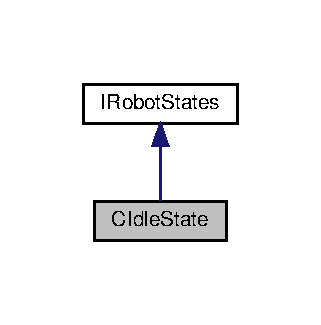
\includegraphics[width=154pt]{classCIdleState__inherit__graph}
\end{center}
\end{figure}


Collaboration diagram for C\+Idle\+State\+:\nopagebreak
\begin{figure}[H]
\begin{center}
\leavevmode
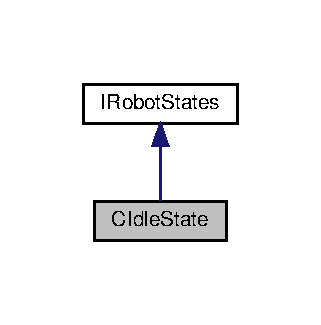
\includegraphics[width=154pt]{classCIdleState__coll__graph}
\end{center}
\end{figure}
\subsection*{Public Member Functions}
\begin{DoxyCompactItemize}
\item 
\hyperlink{classCIdleState_a644c79b15da13871f33656e34ee30c45}{C\+Idle\+State} (\hyperlink{classCEvent}{C\+Event} \&r\+Event, std\+::shared\+\_\+ptr$<$ \hyperlink{classCConfiguration}{C\+Configuration} $>$ sp\+Configuration)
\begin{DoxyCompactList}\small\item\em The state a new Robot\+Arm\+Controller is in and its in while it is idle. \end{DoxyCompactList}\item 
void \hyperlink{classCIdleState_afcfc7e601c50b99c27380b9541fc3795}{Entry} ()
\begin{DoxyCompactList}\small\item\em the entry action which will be executed for the various states when the context enters that state. \end{DoxyCompactList}\item 
void \hyperlink{classCIdleState_a7ae1fe9a96dfb78faaebd068bb8ecae7}{Do} ()
\begin{DoxyCompactList}\small\item\em The do activity which will be executed after the entry action for the various states when the context enters that state. \end{DoxyCompactList}\item 
void \hyperlink{classCIdleState_a634bf12d9a7f29504c7dc6df7d419835}{Exit} ()
\begin{DoxyCompactList}\small\item\em The exit action which will executed when the context transitions off of the state. \end{DoxyCompactList}\item 
void \hyperlink{classCIdleState_a12d0c6b590c56cdc9018524d632d4871}{Handle\+Event} (\hyperlink{classCEvent}{C\+Event} \&r\+Event, \hyperlink{classCRobotContext}{C\+Robot\+Context} \&r\+Context)
\begin{DoxyCompactList}\small\item\em The Handle\+Event function defines how the context will react to the next event, this depends on the state it is currently in. \end{DoxyCompactList}\end{DoxyCompactItemize}


\subsection{Constructor \& Destructor Documentation}
\mbox{\Hypertarget{classCIdleState_a644c79b15da13871f33656e34ee30c45}\label{classCIdleState_a644c79b15da13871f33656e34ee30c45}} 
\index{C\+Idle\+State@{C\+Idle\+State}!C\+Idle\+State@{C\+Idle\+State}}
\index{C\+Idle\+State@{C\+Idle\+State}!C\+Idle\+State@{C\+Idle\+State}}
\subsubsection{\texorpdfstring{C\+Idle\+State()}{CIdleState()}}
{\footnotesize\ttfamily C\+Idle\+State\+::\+C\+Idle\+State (\begin{DoxyParamCaption}\item[{\hyperlink{classCEvent}{C\+Event} \&}]{r\+Event,  }\item[{std\+::shared\+\_\+ptr$<$ \hyperlink{classCConfiguration}{C\+Configuration} $>$}]{sp\+Configuration }\end{DoxyParamCaption})}



The state a new Robot\+Arm\+Controller is in and its in while it is idle. 


\begin{DoxyParams}{Parameters}
{\em r\+Event} & The event that triggered this state \\
\hline
{\em sp\+Configuration} & the Configuration with the calibrated values for the robotarm, this will be passed when the handle\+Event function is called onto other states. \\
\hline
\end{DoxyParams}


\subsection{Member Function Documentation}
\mbox{\Hypertarget{classCIdleState_a7ae1fe9a96dfb78faaebd068bb8ecae7}\label{classCIdleState_a7ae1fe9a96dfb78faaebd068bb8ecae7}} 
\index{C\+Idle\+State@{C\+Idle\+State}!Do@{Do}}
\index{Do@{Do}!C\+Idle\+State@{C\+Idle\+State}}
\subsubsection{\texorpdfstring{Do()}{Do()}}
{\footnotesize\ttfamily void C\+Idle\+State\+::\+Do (\begin{DoxyParamCaption}{ }\end{DoxyParamCaption})\hspace{0.3cm}{\ttfamily [virtual]}}



The do activity which will be executed after the entry action for the various states when the context enters that state. 



Implements \hyperlink{classIRobotStates_aa681381e72738a2870c3f13f552a2e93}{I\+Robot\+States}.

\mbox{\Hypertarget{classCIdleState_afcfc7e601c50b99c27380b9541fc3795}\label{classCIdleState_afcfc7e601c50b99c27380b9541fc3795}} 
\index{C\+Idle\+State@{C\+Idle\+State}!Entry@{Entry}}
\index{Entry@{Entry}!C\+Idle\+State@{C\+Idle\+State}}
\subsubsection{\texorpdfstring{Entry()}{Entry()}}
{\footnotesize\ttfamily void C\+Idle\+State\+::\+Entry (\begin{DoxyParamCaption}{ }\end{DoxyParamCaption})\hspace{0.3cm}{\ttfamily [virtual]}}



the entry action which will be executed for the various states when the context enters that state. 



Implements \hyperlink{classIRobotStates_af43ddb52f5100b42c3d11b71fb1f10dd}{I\+Robot\+States}.

\mbox{\Hypertarget{classCIdleState_a634bf12d9a7f29504c7dc6df7d419835}\label{classCIdleState_a634bf12d9a7f29504c7dc6df7d419835}} 
\index{C\+Idle\+State@{C\+Idle\+State}!Exit@{Exit}}
\index{Exit@{Exit}!C\+Idle\+State@{C\+Idle\+State}}
\subsubsection{\texorpdfstring{Exit()}{Exit()}}
{\footnotesize\ttfamily void C\+Idle\+State\+::\+Exit (\begin{DoxyParamCaption}{ }\end{DoxyParamCaption})\hspace{0.3cm}{\ttfamily [virtual]}}



The exit action which will executed when the context transitions off of the state. 



Implements \hyperlink{classIRobotStates_a099417875e67f047ca38e08890491529}{I\+Robot\+States}.

\mbox{\Hypertarget{classCIdleState_a12d0c6b590c56cdc9018524d632d4871}\label{classCIdleState_a12d0c6b590c56cdc9018524d632d4871}} 
\index{C\+Idle\+State@{C\+Idle\+State}!Handle\+Event@{Handle\+Event}}
\index{Handle\+Event@{Handle\+Event}!C\+Idle\+State@{C\+Idle\+State}}
\subsubsection{\texorpdfstring{Handle\+Event()}{HandleEvent()}}
{\footnotesize\ttfamily void C\+Idle\+State\+::\+Handle\+Event (\begin{DoxyParamCaption}\item[{\hyperlink{classCEvent}{C\+Event} \&}]{r\+Event,  }\item[{\hyperlink{classCRobotContext}{C\+Robot\+Context} \&}]{r\+Context }\end{DoxyParamCaption})\hspace{0.3cm}{\ttfamily [virtual]}}



The Handle\+Event function defines how the context will react to the next event, this depends on the state it is currently in. 


\begin{DoxyParams}{Parameters}
{\em r\+Event} & The next event to be handle by the state machine \\
\hline
{\em r\+Context} & The context which will go through a state because of the incoming event. \\
\hline
\end{DoxyParams}


Implements \hyperlink{classIRobotStates_a0b6c28a3deed04f93371a9395022f1ed}{I\+Robot\+States}.



The documentation for this class was generated from the following files\+:\begin{DoxyCompactItemize}
\item 
\hyperlink{CStates_8h}{C\+States.\+h}\item 
C\+States.\+cpp\end{DoxyCompactItemize}

\hypertarget{classCMove}{}\section{C\+Move Class Reference}
\label{classCMove}\index{C\+Move@{C\+Move}}
\subsection*{Public Member Functions}
\begin{DoxyCompactItemize}
\item 
\mbox{\Hypertarget{classCMove_a49dbf1de9a8eadbf9ea8b1929ca3e626}\label{classCMove_a49dbf1de9a8eadbf9ea8b1929ca3e626}} 
{\bfseries C\+Move} (std\+::shared\+\_\+ptr$<$ \hyperlink{classCConfiguration}{C\+Configuration} $>$ sp\+Configuration)
\item 
void \hyperlink{classCMove_a0c7bf10c045b4369b0d32a63d93ed990}{Execute} (e\+Command e\+Command, std\+::vector$<$ std\+::shared\+\_\+ptr$<$ \hyperlink{classCServoInstruction}{C\+Servo\+Instruction} $>$$>$ r\+Servo\+Instructions)
\begin{DoxyCompactList}\small\item\em Executes servo commands and ultimately moves the robotarm when instructions are valid. \end{DoxyCompactList}\item 
void \hyperlink{classCMove_a9fdfeec108cc173657146525cdf48824}{Execute\+Calibrate} (e\+Command e\+Command, std\+::vector$<$ std\+::shared\+\_\+ptr$<$ \hyperlink{classCServoInstruction}{C\+Servo\+Instruction} $>$$>$ r\+Servo\+Instructions)
\begin{DoxyCompactList}\small\item\em Executes servo commands and ultimately moves the robotarm when instructions are valid. Using this function will set the values in the robotarms configuration when they surpass current boundries. \end{DoxyCompactList}\item 
bool \hyperlink{classCMove_a42a503487eb0aeed688fad00e18c8071}{Is\+Instruction\+Valid} (std\+::shared\+\_\+ptr$<$ \hyperlink{classCServoInstruction}{C\+Servo\+Instruction} $>$ r\+Servo\+Instruction)
\begin{DoxyCompactList}\small\item\em Checks the validity of servo instructions based on the minimal angle and maximum angle of the servo\textquotesingle{}s. \end{DoxyCompactList}\item 
uint16\+\_\+t \hyperlink{classCMove_a716dede77aa60e3b3254f1d436cf2c40}{Degrees\+To\+P\+WM} (e\+Servos servo, int16\+\_\+t degrees)
\begin{DoxyCompactList}\small\item\em Calculates the degrees, commonly stored in servoinstructions, to P\+WM for a specific servo based on its ranges. \end{DoxyCompactList}\item 
uint16\+\_\+t \hyperlink{classCMove_ace7c94d5da8fed1ae1f9cad3d17bba3f}{Calibration\+Degrees\+To\+Pwm} (int16\+\_\+t degrees)
\begin{DoxyCompactList}\small\item\em Calculates the degrees, commonly storedd in servoinstructions, to P\+WM for a specific servo based on its ranges. This function is used when commanding the robotarm during calibration. For this calculation a standardised set of upper and lower limits is used. \end{DoxyCompactList}\item 
std\+::vector$<$ int $>$ \hyperlink{classCMove_ae34b579c70c71a761af9245db1b7571e}{Get\+Min\+And\+Max\+Value} (std\+::shared\+\_\+ptr$<$ \hyperlink{classCServoInstruction}{C\+Servo\+Instruction} $>$ instruction)
\begin{DoxyCompactList}\small\item\em This function gets the upper and lower limit for a servo which has an instruction for it. \end{DoxyCompactList}\end{DoxyCompactItemize}


\subsection{Member Function Documentation}
\mbox{\Hypertarget{classCMove_ace7c94d5da8fed1ae1f9cad3d17bba3f}\label{classCMove_ace7c94d5da8fed1ae1f9cad3d17bba3f}} 
\index{C\+Move@{C\+Move}!Calibration\+Degrees\+To\+Pwm@{Calibration\+Degrees\+To\+Pwm}}
\index{Calibration\+Degrees\+To\+Pwm@{Calibration\+Degrees\+To\+Pwm}!C\+Move@{C\+Move}}
\subsubsection{\texorpdfstring{Calibration\+Degrees\+To\+Pwm()}{CalibrationDegreesToPwm()}}
{\footnotesize\ttfamily uint16\+\_\+t C\+Move\+::\+Calibration\+Degrees\+To\+Pwm (\begin{DoxyParamCaption}\item[{int16\+\_\+t}]{degrees }\end{DoxyParamCaption})}



Calculates the degrees, commonly storedd in servoinstructions, to P\+WM for a specific servo based on its ranges. This function is used when commanding the robotarm during calibration. For this calculation a standardised set of upper and lower limits is used. 


\begin{DoxyParams}{Parameters}
{\em degrees} & the degrees to be translated to P\+WM \\
\hline
\end{DoxyParams}
\begin{DoxyReturn}{Returns}
uint16\+\_\+t the P\+WM which matches the degrees 
\end{DoxyReturn}
\mbox{\Hypertarget{classCMove_a716dede77aa60e3b3254f1d436cf2c40}\label{classCMove_a716dede77aa60e3b3254f1d436cf2c40}} 
\index{C\+Move@{C\+Move}!Degrees\+To\+P\+WM@{Degrees\+To\+P\+WM}}
\index{Degrees\+To\+P\+WM@{Degrees\+To\+P\+WM}!C\+Move@{C\+Move}}
\subsubsection{\texorpdfstring{Degrees\+To\+P\+W\+M()}{DegreesToPWM()}}
{\footnotesize\ttfamily uint16\+\_\+t C\+Move\+::\+Degrees\+To\+P\+WM (\begin{DoxyParamCaption}\item[{e\+Servos}]{servo,  }\item[{int16\+\_\+t}]{degrees }\end{DoxyParamCaption})}



Calculates the degrees, commonly stored in servoinstructions, to P\+WM for a specific servo based on its ranges. 


\begin{DoxyParams}{Parameters}
{\em servo} & the servo whose minimum and maximum values will be used in the calculation \\
\hline
{\em degrees} & the degrees which will de rewritten into P\+WM \\
\hline
\end{DoxyParams}
\begin{DoxyReturn}{Returns}
uint16\+\_\+t returns the amount of P\+WM that matches the degrees 
\end{DoxyReturn}
\mbox{\Hypertarget{classCMove_a0c7bf10c045b4369b0d32a63d93ed990}\label{classCMove_a0c7bf10c045b4369b0d32a63d93ed990}} 
\index{C\+Move@{C\+Move}!Execute@{Execute}}
\index{Execute@{Execute}!C\+Move@{C\+Move}}
\subsubsection{\texorpdfstring{Execute()}{Execute()}}
{\footnotesize\ttfamily void C\+Move\+::\+Execute (\begin{DoxyParamCaption}\item[{e\+Command}]{e\+Command,  }\item[{std\+::vector$<$ std\+::shared\+\_\+ptr$<$ \hyperlink{classCServoInstruction}{C\+Servo\+Instruction} $>$$>$}]{r\+Servo\+Instructions }\end{DoxyParamCaption})}



Executes servo commands and ultimately moves the robotarm when instructions are valid. 


\begin{DoxyParams}{Parameters}
{\em e\+Command} & the type of command to be executed by the robotarm \\
\hline
{\em r\+Servo\+Instructions} & a list of instructions for the different servos \\
\hline
\end{DoxyParams}
\mbox{\Hypertarget{classCMove_a9fdfeec108cc173657146525cdf48824}\label{classCMove_a9fdfeec108cc173657146525cdf48824}} 
\index{C\+Move@{C\+Move}!Execute\+Calibrate@{Execute\+Calibrate}}
\index{Execute\+Calibrate@{Execute\+Calibrate}!C\+Move@{C\+Move}}
\subsubsection{\texorpdfstring{Execute\+Calibrate()}{ExecuteCalibrate()}}
{\footnotesize\ttfamily void C\+Move\+::\+Execute\+Calibrate (\begin{DoxyParamCaption}\item[{e\+Command}]{e\+Command,  }\item[{std\+::vector$<$ std\+::shared\+\_\+ptr$<$ \hyperlink{classCServoInstruction}{C\+Servo\+Instruction} $>$$>$}]{r\+Servo\+Instructions }\end{DoxyParamCaption})}



Executes servo commands and ultimately moves the robotarm when instructions are valid. Using this function will set the values in the robotarms configuration when they surpass current boundries. 


\begin{DoxyParams}{Parameters}
{\em e\+Command} & the type of command to be executed by the robotarm(usually C\+A\+L\+I\+B\+R\+A\+T\+E\+\_\+\+C\+O\+M\+M\+A\+N\+D) \\
\hline
{\em r\+Servo\+Instructions} & a list of instructions for the different servos \\
\hline
\end{DoxyParams}
\mbox{\Hypertarget{classCMove_ae34b579c70c71a761af9245db1b7571e}\label{classCMove_ae34b579c70c71a761af9245db1b7571e}} 
\index{C\+Move@{C\+Move}!Get\+Min\+And\+Max\+Value@{Get\+Min\+And\+Max\+Value}}
\index{Get\+Min\+And\+Max\+Value@{Get\+Min\+And\+Max\+Value}!C\+Move@{C\+Move}}
\subsubsection{\texorpdfstring{Get\+Min\+And\+Max\+Value()}{GetMinAndMaxValue()}}
{\footnotesize\ttfamily std\+::vector$<$ int $>$ C\+Move\+::\+Get\+Min\+And\+Max\+Value (\begin{DoxyParamCaption}\item[{std\+::shared\+\_\+ptr$<$ \hyperlink{classCServoInstruction}{C\+Servo\+Instruction} $>$}]{instruction }\end{DoxyParamCaption})}



This function gets the upper and lower limit for a servo which has an instruction for it. 


\begin{DoxyParams}{Parameters}
{\em instruction} & the instruction for a specific servo \\
\hline
\end{DoxyParams}
\begin{DoxyReturn}{Returns}
std\+::vector$<$int$>$ the lower limit of the servo followed by the upper limit of the servo. 
\end{DoxyReturn}
\mbox{\Hypertarget{classCMove_a42a503487eb0aeed688fad00e18c8071}\label{classCMove_a42a503487eb0aeed688fad00e18c8071}} 
\index{C\+Move@{C\+Move}!Is\+Instruction\+Valid@{Is\+Instruction\+Valid}}
\index{Is\+Instruction\+Valid@{Is\+Instruction\+Valid}!C\+Move@{C\+Move}}
\subsubsection{\texorpdfstring{Is\+Instruction\+Valid()}{IsInstructionValid()}}
{\footnotesize\ttfamily bool C\+Move\+::\+Is\+Instruction\+Valid (\begin{DoxyParamCaption}\item[{std\+::shared\+\_\+ptr$<$ \hyperlink{classCServoInstruction}{C\+Servo\+Instruction} $>$}]{r\+Servo\+Instruction }\end{DoxyParamCaption})}



Checks the validity of servo instructions based on the minimal angle and maximum angle of the servo\textquotesingle{}s. 


\begin{DoxyParams}{Parameters}
{\em r\+Servo\+Instruction} & the servoinstruction which will be tested for it\textquotesingle{}s validity \\
\hline
\end{DoxyParams}
\begin{DoxyReturn}{Returns}
true Returns true if the instruction is valid 

false Returns false if the instruction is invalid 
\end{DoxyReturn}


The documentation for this class was generated from the following files\+:\begin{DoxyCompactItemize}
\item 
Robot\+High\+Level/\hyperlink{CMove_8h}{C\+Move.\+h}\item 
Robot\+High\+Level/\hyperlink{CMove_8cpp}{C\+Move.\+cpp}\end{DoxyCompactItemize}

\hypertarget{classCMoveState}{}\section{C\+Move\+State Class Reference}
\label{classCMoveState}\index{C\+Move\+State@{C\+Move\+State}}


Inheritance diagram for C\+Move\+State\+:\nopagebreak
\begin{figure}[H]
\begin{center}
\leavevmode
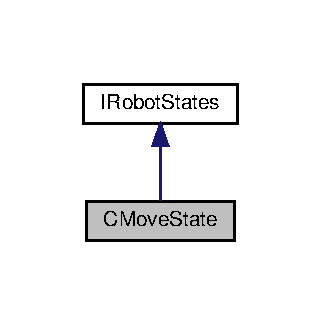
\includegraphics[width=154pt]{classCMoveState__inherit__graph}
\end{center}
\end{figure}


Collaboration diagram for C\+Move\+State\+:\nopagebreak
\begin{figure}[H]
\begin{center}
\leavevmode
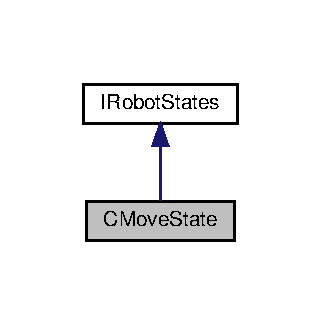
\includegraphics[width=154pt]{classCMoveState__coll__graph}
\end{center}
\end{figure}
\subsection*{Public Member Functions}
\begin{DoxyCompactItemize}
\item 
\hyperlink{classCMoveState_a3b1e230eb78db6e622687ba3b73db8e4}{C\+Move\+State} (\hyperlink{classCEvent}{C\+Event} \&r\+Event, std\+::shared\+\_\+ptr$<$ \hyperlink{classCConfiguration}{C\+Configuration} $>$ sp\+Configuration)
\begin{DoxyCompactList}\small\item\em The state a Robot\+Arm\+Controller is in when it recieves and executes a move command. \end{DoxyCompactList}\item 
void \hyperlink{classCMoveState_ae9bda8d64d42c16e19facdfa8eb842e2}{Entry} ()
\begin{DoxyCompactList}\small\item\em the entry action which will be executed for the various states when the context enters that state. \end{DoxyCompactList}\item 
void \hyperlink{classCMoveState_acd364df1357b25ee616a7444116cf9f6}{Do} ()
\begin{DoxyCompactList}\small\item\em The do activity which will be executed after the entry action for the various states when the context enters that state. \end{DoxyCompactList}\item 
void \hyperlink{classCMoveState_ac6f27ce9a561ab6baf297e106d3f346d}{Exit} ()
\begin{DoxyCompactList}\small\item\em The exit action which will executed when the context transitions off of the state. \end{DoxyCompactList}\item 
void \hyperlink{classCMoveState_a49c6051142c4839e1a512f38859589ad}{Handle\+Event} (\hyperlink{classCEvent}{C\+Event} \&r\+Event, \hyperlink{classCRobotContext}{C\+Robot\+Context} \&r\+Context)
\begin{DoxyCompactList}\small\item\em The Handle\+Event function defines how the context will react to the next event, this depends on the state it is currently in. \end{DoxyCompactList}\end{DoxyCompactItemize}


\subsection{Constructor \& Destructor Documentation}
\mbox{\Hypertarget{classCMoveState_a3b1e230eb78db6e622687ba3b73db8e4}\label{classCMoveState_a3b1e230eb78db6e622687ba3b73db8e4}} 
\index{C\+Move\+State@{C\+Move\+State}!C\+Move\+State@{C\+Move\+State}}
\index{C\+Move\+State@{C\+Move\+State}!C\+Move\+State@{C\+Move\+State}}
\subsubsection{\texorpdfstring{C\+Move\+State()}{CMoveState()}}
{\footnotesize\ttfamily C\+Move\+State\+::\+C\+Move\+State (\begin{DoxyParamCaption}\item[{\hyperlink{classCEvent}{C\+Event} \&}]{r\+Event,  }\item[{std\+::shared\+\_\+ptr$<$ \hyperlink{classCConfiguration}{C\+Configuration} $>$}]{sp\+Configuration }\end{DoxyParamCaption})}



The state a Robot\+Arm\+Controller is in when it recieves and executes a move command. 


\begin{DoxyParams}{Parameters}
{\em r\+Event} & The event that triggered this state \\
\hline
{\em sp\+Configuration} & the Configuration with the calibrated values for the robotarm, this will be passed when the handle\+Event function is called onto other states. \\
\hline
\end{DoxyParams}


\subsection{Member Function Documentation}
\mbox{\Hypertarget{classCMoveState_acd364df1357b25ee616a7444116cf9f6}\label{classCMoveState_acd364df1357b25ee616a7444116cf9f6}} 
\index{C\+Move\+State@{C\+Move\+State}!Do@{Do}}
\index{Do@{Do}!C\+Move\+State@{C\+Move\+State}}
\subsubsection{\texorpdfstring{Do()}{Do()}}
{\footnotesize\ttfamily void C\+Move\+State\+::\+Do (\begin{DoxyParamCaption}{ }\end{DoxyParamCaption})\hspace{0.3cm}{\ttfamily [virtual]}}



The do activity which will be executed after the entry action for the various states when the context enters that state. 



Implements \hyperlink{classIRobotStates_aa681381e72738a2870c3f13f552a2e93}{I\+Robot\+States}.

\mbox{\Hypertarget{classCMoveState_ae9bda8d64d42c16e19facdfa8eb842e2}\label{classCMoveState_ae9bda8d64d42c16e19facdfa8eb842e2}} 
\index{C\+Move\+State@{C\+Move\+State}!Entry@{Entry}}
\index{Entry@{Entry}!C\+Move\+State@{C\+Move\+State}}
\subsubsection{\texorpdfstring{Entry()}{Entry()}}
{\footnotesize\ttfamily void C\+Move\+State\+::\+Entry (\begin{DoxyParamCaption}{ }\end{DoxyParamCaption})\hspace{0.3cm}{\ttfamily [virtual]}}



the entry action which will be executed for the various states when the context enters that state. 



Implements \hyperlink{classIRobotStates_af43ddb52f5100b42c3d11b71fb1f10dd}{I\+Robot\+States}.

\mbox{\Hypertarget{classCMoveState_ac6f27ce9a561ab6baf297e106d3f346d}\label{classCMoveState_ac6f27ce9a561ab6baf297e106d3f346d}} 
\index{C\+Move\+State@{C\+Move\+State}!Exit@{Exit}}
\index{Exit@{Exit}!C\+Move\+State@{C\+Move\+State}}
\subsubsection{\texorpdfstring{Exit()}{Exit()}}
{\footnotesize\ttfamily void C\+Move\+State\+::\+Exit (\begin{DoxyParamCaption}{ }\end{DoxyParamCaption})\hspace{0.3cm}{\ttfamily [virtual]}}



The exit action which will executed when the context transitions off of the state. 



Implements \hyperlink{classIRobotStates_a099417875e67f047ca38e08890491529}{I\+Robot\+States}.

\mbox{\Hypertarget{classCMoveState_a49c6051142c4839e1a512f38859589ad}\label{classCMoveState_a49c6051142c4839e1a512f38859589ad}} 
\index{C\+Move\+State@{C\+Move\+State}!Handle\+Event@{Handle\+Event}}
\index{Handle\+Event@{Handle\+Event}!C\+Move\+State@{C\+Move\+State}}
\subsubsection{\texorpdfstring{Handle\+Event()}{HandleEvent()}}
{\footnotesize\ttfamily void C\+Move\+State\+::\+Handle\+Event (\begin{DoxyParamCaption}\item[{\hyperlink{classCEvent}{C\+Event} \&}]{r\+Event,  }\item[{\hyperlink{classCRobotContext}{C\+Robot\+Context} \&}]{r\+Context }\end{DoxyParamCaption})\hspace{0.3cm}{\ttfamily [virtual]}}



The Handle\+Event function defines how the context will react to the next event, this depends on the state it is currently in. 


\begin{DoxyParams}{Parameters}
{\em r\+Event} & The next event to be handle by the state machine \\
\hline
{\em r\+Context} & The context which will go through a state because of the incoming event. \\
\hline
\end{DoxyParams}


Implements \hyperlink{classIRobotStates_a0b6c28a3deed04f93371a9395022f1ed}{I\+Robot\+States}.



The documentation for this class was generated from the following files\+:\begin{DoxyCompactItemize}
\item 
\hyperlink{CStates_8h}{C\+States.\+h}\item 
C\+States.\+cpp\end{DoxyCompactItemize}

\hypertarget{classCRobotContext}{}\section{C\+Robot\+Context Class Reference}
\label{classCRobotContext}\index{C\+Robot\+Context@{C\+Robot\+Context}}
\subsection*{Public Member Functions}
\begin{DoxyCompactItemize}
\item 
void \hyperlink{classCRobotContext_af50652269de0b3977920d97345ac3606}{Run} ()
\begin{DoxyCompactList}\small\item\em The Run function runs the state machine so it handles all the events in its queue, afterwards it will stay waiting for new events to be created by functions to be called by ros. \end{DoxyCompactList}\item 
void \hyperlink{classCRobotContext_a34c126d70c235c1fdd60d028aea523d7}{Set\+State} (std\+::shared\+\_\+ptr$<$ \hyperlink{classIRobotStates}{I\+Robot\+States} $>$ sp\+\_\+state)
\begin{DoxyCompactList}\small\item\em Sets the state of the Context, in doing so it goes through the exit action of the previous state, the entry action of the new state and into the do activity of the new state. All in that order. \end{DoxyCompactList}\item 
void \hyperlink{classCRobotContext_a0c691e094641e2e424dce4505a5db275}{Move\+Callback} (const Robot\+Arm\+Controller\+::\+Move\+::\+Const\+Ptr \&move\+Msg)
\begin{DoxyCompactList}\small\item\em The callback function which will be called when a message gets posted on the /\+Robot\+Arm\+Controller/\+Move ros topic. \end{DoxyCompactList}\item 
void \hyperlink{classCRobotContext_a64c5bcd86ffe2d1dff1354187f8e165b}{Calibrate\+Callback} (const Robot\+Arm\+Controller\+::\+Move\+::\+Const\+Ptr \&calibrate\+Msg)
\begin{DoxyCompactList}\small\item\em The callback function which will be called when a message gets posted on the /\+Robot\+Arm\+Controller/\+Calibrate ros topic. \end{DoxyCompactList}\item 
void \hyperlink{classCRobotContext_ab4f5e962e8b722b8e844e41c64831ea9}{Emergency\+Stop\+Callback} (const Robot\+Arm\+Controller\+::\+Emergency\+Stop\+::\+Const\+Ptr \&stop\+Msg)
\begin{DoxyCompactList}\small\item\em The callback function which will be called when a message gets posted on the /\+Robot\+Arm\+Controller/\+Emergency\+Stop ros topic. \end{DoxyCompactList}\item 
void \hyperlink{classCRobotContext_a9ab9301b43253d237984667c1b586cec}{Programmed\+Position\+Callback} (const Robot\+Arm\+Controller\+::\+Programmed\+Position\+::\+Const\+Ptr \&programmed\+Position\+Msg)
\begin{DoxyCompactList}\small\item\em The callback function which will be called when a message gets posted on the /\+Robot\+Arm\+Controller/\+Programmed\+Position ros topic. \end{DoxyCompactList}\end{DoxyCompactItemize}


\subsection{Member Function Documentation}
\mbox{\Hypertarget{classCRobotContext_a64c5bcd86ffe2d1dff1354187f8e165b}\label{classCRobotContext_a64c5bcd86ffe2d1dff1354187f8e165b}} 
\index{C\+Robot\+Context@{C\+Robot\+Context}!Calibrate\+Callback@{Calibrate\+Callback}}
\index{Calibrate\+Callback@{Calibrate\+Callback}!C\+Robot\+Context@{C\+Robot\+Context}}
\subsubsection{\texorpdfstring{Calibrate\+Callback()}{CalibrateCallback()}}
{\footnotesize\ttfamily void C\+Robot\+Context\+::\+Calibrate\+Callback (\begin{DoxyParamCaption}\item[{const Robot\+Arm\+Controller\+::\+Move\+::\+Const\+Ptr \&}]{calibrate\+Msg }\end{DoxyParamCaption})}



The callback function which will be called when a message gets posted on the /\+Robot\+Arm\+Controller/\+Calibrate ros topic. 


\begin{DoxyParams}{Parameters}
{\em calibrate\+Msg} & a message containing instructions for the individual servos of the robotarm. these values will be used to calibrate new boundries \\
\hline
\end{DoxyParams}
\mbox{\Hypertarget{classCRobotContext_ab4f5e962e8b722b8e844e41c64831ea9}\label{classCRobotContext_ab4f5e962e8b722b8e844e41c64831ea9}} 
\index{C\+Robot\+Context@{C\+Robot\+Context}!Emergency\+Stop\+Callback@{Emergency\+Stop\+Callback}}
\index{Emergency\+Stop\+Callback@{Emergency\+Stop\+Callback}!C\+Robot\+Context@{C\+Robot\+Context}}
\subsubsection{\texorpdfstring{Emergency\+Stop\+Callback()}{EmergencyStopCallback()}}
{\footnotesize\ttfamily void C\+Robot\+Context\+::\+Emergency\+Stop\+Callback (\begin{DoxyParamCaption}\item[{const Robot\+Arm\+Controller\+::\+Emergency\+Stop\+::\+Const\+Ptr \&}]{stop\+Msg }\end{DoxyParamCaption})}



The callback function which will be called when a message gets posted on the /\+Robot\+Arm\+Controller/\+Emergency\+Stop ros topic. 


\begin{DoxyParams}{Parameters}
{\em stop\+Msg} & an empty message \\
\hline
\end{DoxyParams}
\mbox{\Hypertarget{classCRobotContext_a0c691e094641e2e424dce4505a5db275}\label{classCRobotContext_a0c691e094641e2e424dce4505a5db275}} 
\index{C\+Robot\+Context@{C\+Robot\+Context}!Move\+Callback@{Move\+Callback}}
\index{Move\+Callback@{Move\+Callback}!C\+Robot\+Context@{C\+Robot\+Context}}
\subsubsection{\texorpdfstring{Move\+Callback()}{MoveCallback()}}
{\footnotesize\ttfamily void C\+Robot\+Context\+::\+Move\+Callback (\begin{DoxyParamCaption}\item[{const Robot\+Arm\+Controller\+::\+Move\+::\+Const\+Ptr \&}]{move\+Msg }\end{DoxyParamCaption})}



The callback function which will be called when a message gets posted on the /\+Robot\+Arm\+Controller/\+Move ros topic. 


\begin{DoxyParams}{Parameters}
{\em move\+Msg} & a message containing instructions for the individual servos of the robotarm \\
\hline
\end{DoxyParams}
\mbox{\Hypertarget{classCRobotContext_a9ab9301b43253d237984667c1b586cec}\label{classCRobotContext_a9ab9301b43253d237984667c1b586cec}} 
\index{C\+Robot\+Context@{C\+Robot\+Context}!Programmed\+Position\+Callback@{Programmed\+Position\+Callback}}
\index{Programmed\+Position\+Callback@{Programmed\+Position\+Callback}!C\+Robot\+Context@{C\+Robot\+Context}}
\subsubsection{\texorpdfstring{Programmed\+Position\+Callback()}{ProgrammedPositionCallback()}}
{\footnotesize\ttfamily void C\+Robot\+Context\+::\+Programmed\+Position\+Callback (\begin{DoxyParamCaption}\item[{const Robot\+Arm\+Controller\+::\+Programmed\+Position\+::\+Const\+Ptr \&}]{programmed\+Position\+Msg }\end{DoxyParamCaption})}



The callback function which will be called when a message gets posted on the /\+Robot\+Arm\+Controller/\+Programmed\+Position ros topic. 


\begin{DoxyParams}{Parameters}
{\em programmed\+Position\+Msg} & a message containing a string to set pre defined positions \\
\hline
\end{DoxyParams}
\mbox{\Hypertarget{classCRobotContext_af50652269de0b3977920d97345ac3606}\label{classCRobotContext_af50652269de0b3977920d97345ac3606}} 
\index{C\+Robot\+Context@{C\+Robot\+Context}!Run@{Run}}
\index{Run@{Run}!C\+Robot\+Context@{C\+Robot\+Context}}
\subsubsection{\texorpdfstring{Run()}{Run()}}
{\footnotesize\ttfamily void C\+Robot\+Context\+::\+Run (\begin{DoxyParamCaption}{ }\end{DoxyParamCaption})}



The Run function runs the state machine so it handles all the events in its queue, afterwards it will stay waiting for new events to be created by functions to be called by ros. 

\mbox{\Hypertarget{classCRobotContext_a34c126d70c235c1fdd60d028aea523d7}\label{classCRobotContext_a34c126d70c235c1fdd60d028aea523d7}} 
\index{C\+Robot\+Context@{C\+Robot\+Context}!Set\+State@{Set\+State}}
\index{Set\+State@{Set\+State}!C\+Robot\+Context@{C\+Robot\+Context}}
\subsubsection{\texorpdfstring{Set\+State()}{SetState()}}
{\footnotesize\ttfamily void C\+Robot\+Context\+::\+Set\+State (\begin{DoxyParamCaption}\item[{std\+::shared\+\_\+ptr$<$ \hyperlink{classIRobotStates}{I\+Robot\+States} $>$}]{sp\+\_\+state }\end{DoxyParamCaption})}



Sets the state of the Context, in doing so it goes through the exit action of the previous state, the entry action of the new state and into the do activity of the new state. All in that order. 


\begin{DoxyParams}{Parameters}
{\em sp\+\_\+state} & a shared pointer to the new state for this context \\
\hline
\end{DoxyParams}


The documentation for this class was generated from the following files\+:\begin{DoxyCompactItemize}
\item 
\hyperlink{CRobotContext_8h}{C\+Robot\+Context.\+h}\item 
C\+Robot\+Context.\+cpp\end{DoxyCompactItemize}

\hypertarget{classCServoInstruction}{}\section{C\+Servo\+Instruction Class Reference}
\label{classCServoInstruction}\index{C\+Servo\+Instruction@{C\+Servo\+Instruction}}
\subsection*{Public Member Functions}
\begin{DoxyCompactItemize}
\item 
\mbox{\Hypertarget{classCServoInstruction_a8c6c2780cb3fc5266e62e81166758d67}\label{classCServoInstruction_a8c6c2780cb3fc5266e62e81166758d67}} 
{\bfseries C\+Servo\+Instruction} (e\+Servos target\+Servo, int64\+\_\+t position, int64\+\_\+t duration, int64\+\_\+t speed)
\item 
\mbox{\Hypertarget{classCServoInstruction_aecfd99820d481b94e6678b99526c3083}\label{classCServoInstruction_aecfd99820d481b94e6678b99526c3083}} 
e\+Servos {\bfseries Get\+Target\+Servo} ()
\item 
\mbox{\Hypertarget{classCServoInstruction_ad2f3fd01da8266d393610b46dca39679}\label{classCServoInstruction_ad2f3fd01da8266d393610b46dca39679}} 
int64\+\_\+t {\bfseries Get\+Position} ()
\item 
\mbox{\Hypertarget{classCServoInstruction_a3bfffbfc97fafad4a0f4bd89170e4bcc}\label{classCServoInstruction_a3bfffbfc97fafad4a0f4bd89170e4bcc}} 
int64\+\_\+t {\bfseries Get\+Duration} ()
\item 
\mbox{\Hypertarget{classCServoInstruction_a12cf1e7d297f0f5401200353d8c4c53f}\label{classCServoInstruction_a12cf1e7d297f0f5401200353d8c4c53f}} 
int64\+\_\+t {\bfseries Get\+Speed} ()
\end{DoxyCompactItemize}


The documentation for this class was generated from the following files\+:\begin{DoxyCompactItemize}
\item 
\hyperlink{CServoInstruction_8h}{C\+Servo\+Instruction.\+h}\item 
C\+Servo\+Instruction.\+cpp\end{DoxyCompactItemize}

\hypertarget{classCStatePublisher}{}\section{C\+State\+Publisher Class Reference}
\label{classCStatePublisher}\index{C\+State\+Publisher@{C\+State\+Publisher}}
\subsection*{Public Member Functions}
\begin{DoxyCompactItemize}
\item 
void \hyperlink{classCStatePublisher_af7144175e8b6e553a182ef660f37616c}{Publish\+State} (\hyperlink{CStatePublisher_8h_a57ce604a7850ac5988b6182daf162fe9}{e\+Publishable\+States} state)
\begin{DoxyCompactList}\small\item\em Publishes the state on the /\+Robot\+Arm\+Controller/\+Behavioural\+State ros topic. \end{DoxyCompactList}\item 
void \hyperlink{classCStatePublisher_a0c6cde04f7712e68951bd50391c1f53e}{Publish\+Protocol\+State} (\hyperlink{CStatePublisher_8h_a57ce604a7850ac5988b6182daf162fe9}{e\+Publishable\+States} state)
\begin{DoxyCompactList}\small\item\em Publishes the state on the /\+Robot\+Arm\+Controller/\+Protocol\+State ros topic. \end{DoxyCompactList}\end{DoxyCompactItemize}
\subsection*{Static Public Member Functions}
\begin{DoxyCompactItemize}
\item 
static \hyperlink{classCStatePublisher}{C\+State\+Publisher} $\ast$ \hyperlink{classCStatePublisher_a473d257be0334c38511096fe5caded74}{Get\+Instance} ()
\begin{DoxyCompactList}\small\item\em Returns the single instance of the \hyperlink{classCStatePublisher}{C\+State\+Publisher} class. \end{DoxyCompactList}\end{DoxyCompactItemize}


\subsection{Member Function Documentation}
\mbox{\Hypertarget{classCStatePublisher_a473d257be0334c38511096fe5caded74}\label{classCStatePublisher_a473d257be0334c38511096fe5caded74}} 
\index{C\+State\+Publisher@{C\+State\+Publisher}!Get\+Instance@{Get\+Instance}}
\index{Get\+Instance@{Get\+Instance}!C\+State\+Publisher@{C\+State\+Publisher}}
\subsubsection{\texorpdfstring{Get\+Instance()}{GetInstance()}}
{\footnotesize\ttfamily \hyperlink{classCStatePublisher}{C\+State\+Publisher} $\ast$ C\+State\+Publisher\+::\+Get\+Instance (\begin{DoxyParamCaption}{ }\end{DoxyParamCaption})\hspace{0.3cm}{\ttfamily [static]}}



Returns the single instance of the \hyperlink{classCStatePublisher}{C\+State\+Publisher} class. 

\begin{DoxyReturn}{Returns}
C\+State\+Publisher$\ast$ A pointer to the singleton statepublisher 
\end{DoxyReturn}
\mbox{\Hypertarget{classCStatePublisher_a0c6cde04f7712e68951bd50391c1f53e}\label{classCStatePublisher_a0c6cde04f7712e68951bd50391c1f53e}} 
\index{C\+State\+Publisher@{C\+State\+Publisher}!Publish\+Protocol\+State@{Publish\+Protocol\+State}}
\index{Publish\+Protocol\+State@{Publish\+Protocol\+State}!C\+State\+Publisher@{C\+State\+Publisher}}
\subsubsection{\texorpdfstring{Publish\+Protocol\+State()}{PublishProtocolState()}}
{\footnotesize\ttfamily void C\+State\+Publisher\+::\+Publish\+Protocol\+State (\begin{DoxyParamCaption}\item[{\hyperlink{CStatePublisher_8h_a57ce604a7850ac5988b6182daf162fe9}{e\+Publishable\+States}}]{state }\end{DoxyParamCaption})}



Publishes the state on the /\+Robot\+Arm\+Controller/\+Protocol\+State ros topic. 


\begin{DoxyParams}{Parameters}
{\em state} & the state to publish on the before mentioned ros topic \\
\hline
\end{DoxyParams}
\mbox{\Hypertarget{classCStatePublisher_af7144175e8b6e553a182ef660f37616c}\label{classCStatePublisher_af7144175e8b6e553a182ef660f37616c}} 
\index{C\+State\+Publisher@{C\+State\+Publisher}!Publish\+State@{Publish\+State}}
\index{Publish\+State@{Publish\+State}!C\+State\+Publisher@{C\+State\+Publisher}}
\subsubsection{\texorpdfstring{Publish\+State()}{PublishState()}}
{\footnotesize\ttfamily void C\+State\+Publisher\+::\+Publish\+State (\begin{DoxyParamCaption}\item[{\hyperlink{CStatePublisher_8h_a57ce604a7850ac5988b6182daf162fe9}{e\+Publishable\+States}}]{state }\end{DoxyParamCaption})}



Publishes the state on the /\+Robot\+Arm\+Controller/\+Behavioural\+State ros topic. 


\begin{DoxyParams}{Parameters}
{\em state} & the state to publish on the before mentioned ros topic \\
\hline
\end{DoxyParams}


The documentation for this class was generated from the following files\+:\begin{DoxyCompactItemize}
\item 
\hyperlink{CStatePublisher_8h}{C\+State\+Publisher.\+h}\item 
C\+State\+Publisher.\+cpp\end{DoxyCompactItemize}

\hypertarget{classCStopState}{}\section{C\+Stop\+State Class Reference}
\label{classCStopState}\index{C\+Stop\+State@{C\+Stop\+State}}


Inheritance diagram for C\+Stop\+State\+:\nopagebreak
\begin{figure}[H]
\begin{center}
\leavevmode
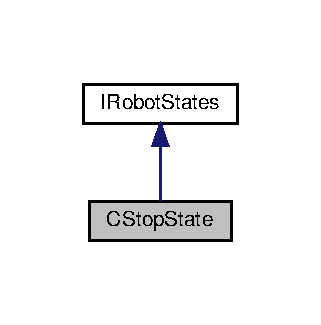
\includegraphics[width=154pt]{classCStopState__inherit__graph}
\end{center}
\end{figure}


Collaboration diagram for C\+Stop\+State\+:\nopagebreak
\begin{figure}[H]
\begin{center}
\leavevmode
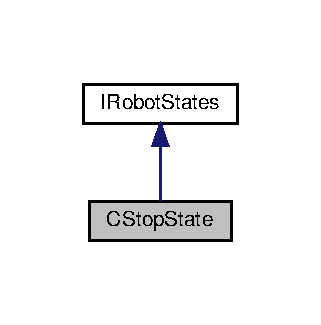
\includegraphics[width=154pt]{classCStopState__coll__graph}
\end{center}
\end{figure}
\subsection*{Public Member Functions}
\begin{DoxyCompactItemize}
\item 
\hyperlink{classCStopState_ac1e10af0a555c8d0df9964d2bf67172c}{C\+Stop\+State} (\hyperlink{classCEvent}{C\+Event} \&r\+Event, std\+::shared\+\_\+ptr$<$ \hyperlink{classCConfiguration}{C\+Configuration} $>$ sp\+Configuration)
\begin{DoxyCompactList}\small\item\em The state a Robot\+Arm\+Controller is in when the emergency stop is used. The application will need to be restarted after the controller is in this state. \end{DoxyCompactList}\item 
void \hyperlink{classCStopState_aae7dbdb7db312f20a16fcd48edc60e83}{Entry} ()
\begin{DoxyCompactList}\small\item\em the entry action which will be executed for the various states when the context enters that state. \end{DoxyCompactList}\item 
void \hyperlink{classCStopState_aba51445ef29e03fa5ffc5cef48923a10}{Do} ()
\begin{DoxyCompactList}\small\item\em The do activity which will be executed after the entry action for the various states when the context enters that state. \end{DoxyCompactList}\item 
void \hyperlink{classCStopState_a2bf7d1e44a9b0c689c86fb00f9684a7b}{Exit} ()
\begin{DoxyCompactList}\small\item\em The exit action which will executed when the context transitions off of the state. \end{DoxyCompactList}\item 
void \hyperlink{classCStopState_abe6af38d9c6b80b98fd78cdb48d7599c}{Handle\+Event} (\hyperlink{classCEvent}{C\+Event} \&r\+Event, \hyperlink{classCRobotContext}{C\+Robot\+Context} \&r\+Context)
\begin{DoxyCompactList}\small\item\em The Handle\+Event function defines how the context will react to the next event, this depends on the state it is currently in. \end{DoxyCompactList}\end{DoxyCompactItemize}


\subsection{Constructor \& Destructor Documentation}
\mbox{\Hypertarget{classCStopState_ac1e10af0a555c8d0df9964d2bf67172c}\label{classCStopState_ac1e10af0a555c8d0df9964d2bf67172c}} 
\index{C\+Stop\+State@{C\+Stop\+State}!C\+Stop\+State@{C\+Stop\+State}}
\index{C\+Stop\+State@{C\+Stop\+State}!C\+Stop\+State@{C\+Stop\+State}}
\subsubsection{\texorpdfstring{C\+Stop\+State()}{CStopState()}}
{\footnotesize\ttfamily C\+Stop\+State\+::\+C\+Stop\+State (\begin{DoxyParamCaption}\item[{\hyperlink{classCEvent}{C\+Event} \&}]{r\+Event,  }\item[{std\+::shared\+\_\+ptr$<$ \hyperlink{classCConfiguration}{C\+Configuration} $>$}]{sp\+Configuration }\end{DoxyParamCaption})}



The state a Robot\+Arm\+Controller is in when the emergency stop is used. The application will need to be restarted after the controller is in this state. 


\begin{DoxyParams}{Parameters}
{\em r\+Event} & The event that triggered this state \\
\hline
{\em sp\+Configuration} & the Configuration with the calibrated values for the robotarm, this will be passed when the handle\+Event function is called onto other states. \\
\hline
\end{DoxyParams}


\subsection{Member Function Documentation}
\mbox{\Hypertarget{classCStopState_aba51445ef29e03fa5ffc5cef48923a10}\label{classCStopState_aba51445ef29e03fa5ffc5cef48923a10}} 
\index{C\+Stop\+State@{C\+Stop\+State}!Do@{Do}}
\index{Do@{Do}!C\+Stop\+State@{C\+Stop\+State}}
\subsubsection{\texorpdfstring{Do()}{Do()}}
{\footnotesize\ttfamily void C\+Stop\+State\+::\+Do (\begin{DoxyParamCaption}{ }\end{DoxyParamCaption})\hspace{0.3cm}{\ttfamily [virtual]}}



The do activity which will be executed after the entry action for the various states when the context enters that state. 



Implements \hyperlink{classIRobotStates_aa681381e72738a2870c3f13f552a2e93}{I\+Robot\+States}.

\mbox{\Hypertarget{classCStopState_aae7dbdb7db312f20a16fcd48edc60e83}\label{classCStopState_aae7dbdb7db312f20a16fcd48edc60e83}} 
\index{C\+Stop\+State@{C\+Stop\+State}!Entry@{Entry}}
\index{Entry@{Entry}!C\+Stop\+State@{C\+Stop\+State}}
\subsubsection{\texorpdfstring{Entry()}{Entry()}}
{\footnotesize\ttfamily void C\+Stop\+State\+::\+Entry (\begin{DoxyParamCaption}{ }\end{DoxyParamCaption})\hspace{0.3cm}{\ttfamily [virtual]}}



the entry action which will be executed for the various states when the context enters that state. 



Implements \hyperlink{classIRobotStates_af43ddb52f5100b42c3d11b71fb1f10dd}{I\+Robot\+States}.

\mbox{\Hypertarget{classCStopState_a2bf7d1e44a9b0c689c86fb00f9684a7b}\label{classCStopState_a2bf7d1e44a9b0c689c86fb00f9684a7b}} 
\index{C\+Stop\+State@{C\+Stop\+State}!Exit@{Exit}}
\index{Exit@{Exit}!C\+Stop\+State@{C\+Stop\+State}}
\subsubsection{\texorpdfstring{Exit()}{Exit()}}
{\footnotesize\ttfamily void C\+Stop\+State\+::\+Exit (\begin{DoxyParamCaption}{ }\end{DoxyParamCaption})\hspace{0.3cm}{\ttfamily [virtual]}}



The exit action which will executed when the context transitions off of the state. 



Implements \hyperlink{classIRobotStates_a099417875e67f047ca38e08890491529}{I\+Robot\+States}.

\mbox{\Hypertarget{classCStopState_abe6af38d9c6b80b98fd78cdb48d7599c}\label{classCStopState_abe6af38d9c6b80b98fd78cdb48d7599c}} 
\index{C\+Stop\+State@{C\+Stop\+State}!Handle\+Event@{Handle\+Event}}
\index{Handle\+Event@{Handle\+Event}!C\+Stop\+State@{C\+Stop\+State}}
\subsubsection{\texorpdfstring{Handle\+Event()}{HandleEvent()}}
{\footnotesize\ttfamily void C\+Stop\+State\+::\+Handle\+Event (\begin{DoxyParamCaption}\item[{\hyperlink{classCEvent}{C\+Event} \&}]{r\+Event,  }\item[{\hyperlink{classCRobotContext}{C\+Robot\+Context} \&}]{r\+Context }\end{DoxyParamCaption})\hspace{0.3cm}{\ttfamily [virtual]}}



The Handle\+Event function defines how the context will react to the next event, this depends on the state it is currently in. 


\begin{DoxyParams}{Parameters}
{\em r\+Event} & The next event to be handle by the state machine \\
\hline
{\em r\+Context} & The context which will go through a state because of the incoming event. \\
\hline
\end{DoxyParams}


Implements \hyperlink{classIRobotStates_a0b6c28a3deed04f93371a9395022f1ed}{I\+Robot\+States}.



The documentation for this class was generated from the following files\+:\begin{DoxyCompactItemize}
\item 
\hyperlink{CStates_8h}{C\+States.\+h}\item 
C\+States.\+cpp\end{DoxyCompactItemize}

\hypertarget{classIExecuteCommand}{}\section{I\+Execute\+Command Class Reference}
\label{classIExecuteCommand}\index{I\+Execute\+Command@{I\+Execute\+Command}}


Inheritance diagram for I\+Execute\+Command\+:\nopagebreak
\begin{figure}[H]
\begin{center}
\leavevmode
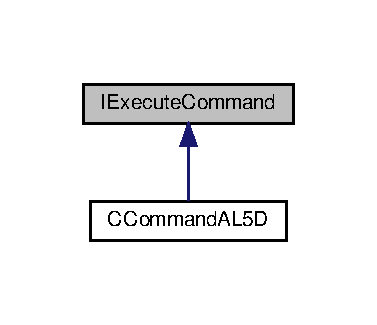
\includegraphics[width=181pt]{classIExecuteCommand__inherit__graph}
\end{center}
\end{figure}
\subsection*{Public Member Functions}
\begin{DoxyCompactItemize}
\item 
virtual void \hyperlink{classIExecuteCommand_a9aaabaf7284c9d295c6e2fdfc1445ca4}{Stop} ()=0
\begin{DoxyCompactList}\small\item\em This function will be called to stop communication to the robotarm. \end{DoxyCompactList}\item 
virtual void \hyperlink{classIExecuteCommand_a266571b3fc97e79be6e00b0df4c5a4ac}{Write} (const std\+::string \&r\+Message)=0
\begin{DoxyCompactList}\small\item\em The write function is called to write a string message to the robotarm. \end{DoxyCompactList}\item 
virtual void \hyperlink{classIExecuteCommand_a0f05e1cf668740504e36de8f662c0864}{Append\+Instruction} (e\+Command e\+Command, int8\+\_\+t servo, int64\+\_\+t position, int64\+\_\+t speed, int64\+\_\+t duration)=0
\begin{DoxyCompactList}\small\item\em the Append\+Instruction function adds an instruction to the list of instructions to send to the robotarm \end{DoxyCompactList}\item 
virtual void \hyperlink{classIExecuteCommand_a8180d6931ffae55f04f9984d45a9c99f}{Execute} ()=0
\begin{DoxyCompactList}\small\item\em The execute function writes the stored instructions as a message to the robotarm. \end{DoxyCompactList}\item 
virtual void \hyperlink{classIExecuteCommand_a34d2dc6186873e0f6f039fd4b41e414a}{Clear\+Lists} ()=0
\begin{DoxyCompactList}\small\item\em The clearlists function clears all the previously appended instructions. \end{DoxyCompactList}\end{DoxyCompactItemize}


\subsection{Member Function Documentation}
\mbox{\Hypertarget{classIExecuteCommand_a0f05e1cf668740504e36de8f662c0864}\label{classIExecuteCommand_a0f05e1cf668740504e36de8f662c0864}} 
\index{I\+Execute\+Command@{I\+Execute\+Command}!Append\+Instruction@{Append\+Instruction}}
\index{Append\+Instruction@{Append\+Instruction}!I\+Execute\+Command@{I\+Execute\+Command}}
\subsubsection{\texorpdfstring{Append\+Instruction()}{AppendInstruction()}}
{\footnotesize\ttfamily virtual void I\+Execute\+Command\+::\+Append\+Instruction (\begin{DoxyParamCaption}\item[{e\+Command}]{e\+Command,  }\item[{int8\+\_\+t}]{servo,  }\item[{int64\+\_\+t}]{position,  }\item[{int64\+\_\+t}]{speed,  }\item[{int64\+\_\+t}]{duration }\end{DoxyParamCaption})\hspace{0.3cm}{\ttfamily [pure virtual]}}



the Append\+Instruction function adds an instruction to the list of instructions to send to the robotarm 


\begin{DoxyParams}{Parameters}
{\em e\+Command} & the type of command to send to the servo \\
\hline
{\em servo} & the servo to control \\
\hline
{\em position} & the position to which the servo has to travel in P\+WM \\
\hline
{\em speed} & the maximum speed of the movement \\
\hline
{\em duration} & the duration of the movement \\
\hline
\end{DoxyParams}


Implemented in \hyperlink{classCCommandAL5D_ae8b75aec364029b7cb65959325b6b9f7}{C\+Command\+A\+L5D}.

\mbox{\Hypertarget{classIExecuteCommand_a34d2dc6186873e0f6f039fd4b41e414a}\label{classIExecuteCommand_a34d2dc6186873e0f6f039fd4b41e414a}} 
\index{I\+Execute\+Command@{I\+Execute\+Command}!Clear\+Lists@{Clear\+Lists}}
\index{Clear\+Lists@{Clear\+Lists}!I\+Execute\+Command@{I\+Execute\+Command}}
\subsubsection{\texorpdfstring{Clear\+Lists()}{ClearLists()}}
{\footnotesize\ttfamily virtual void I\+Execute\+Command\+::\+Clear\+Lists (\begin{DoxyParamCaption}{ }\end{DoxyParamCaption})\hspace{0.3cm}{\ttfamily [pure virtual]}}



The clearlists function clears all the previously appended instructions. 



Implemented in \hyperlink{classCCommandAL5D_a46f133aa4b243af59e02f2cc23b12aa3}{C\+Command\+A\+L5D}.

\mbox{\Hypertarget{classIExecuteCommand_a8180d6931ffae55f04f9984d45a9c99f}\label{classIExecuteCommand_a8180d6931ffae55f04f9984d45a9c99f}} 
\index{I\+Execute\+Command@{I\+Execute\+Command}!Execute@{Execute}}
\index{Execute@{Execute}!I\+Execute\+Command@{I\+Execute\+Command}}
\subsubsection{\texorpdfstring{Execute()}{Execute()}}
{\footnotesize\ttfamily virtual void I\+Execute\+Command\+::\+Execute (\begin{DoxyParamCaption}{ }\end{DoxyParamCaption})\hspace{0.3cm}{\ttfamily [pure virtual]}}



The execute function writes the stored instructions as a message to the robotarm. 



Implemented in \hyperlink{classCCommandAL5D_ac225e1c103a802a9276f201c94281ae2}{C\+Command\+A\+L5D}.

\mbox{\Hypertarget{classIExecuteCommand_a9aaabaf7284c9d295c6e2fdfc1445ca4}\label{classIExecuteCommand_a9aaabaf7284c9d295c6e2fdfc1445ca4}} 
\index{I\+Execute\+Command@{I\+Execute\+Command}!Stop@{Stop}}
\index{Stop@{Stop}!I\+Execute\+Command@{I\+Execute\+Command}}
\subsubsection{\texorpdfstring{Stop()}{Stop()}}
{\footnotesize\ttfamily virtual void I\+Execute\+Command\+::\+Stop (\begin{DoxyParamCaption}{ }\end{DoxyParamCaption})\hspace{0.3cm}{\ttfamily [pure virtual]}}



This function will be called to stop communication to the robotarm. 



Implemented in \hyperlink{classCCommandAL5D_a3cd260bd7bf8b4aa72dacc1d1ef2d38b}{C\+Command\+A\+L5D}.

\mbox{\Hypertarget{classIExecuteCommand_a266571b3fc97e79be6e00b0df4c5a4ac}\label{classIExecuteCommand_a266571b3fc97e79be6e00b0df4c5a4ac}} 
\index{I\+Execute\+Command@{I\+Execute\+Command}!Write@{Write}}
\index{Write@{Write}!I\+Execute\+Command@{I\+Execute\+Command}}
\subsubsection{\texorpdfstring{Write()}{Write()}}
{\footnotesize\ttfamily virtual void I\+Execute\+Command\+::\+Write (\begin{DoxyParamCaption}\item[{const std\+::string \&}]{r\+Message }\end{DoxyParamCaption})\hspace{0.3cm}{\ttfamily [pure virtual]}}



The write function is called to write a string message to the robotarm. 


\begin{DoxyParams}{Parameters}
{\em r\+Message} & the string which will be sent to the robotarm \\
\hline
\end{DoxyParams}


Implemented in \hyperlink{classCCommandAL5D_a308c945d4ed4009c85158a72e5db1bd5}{C\+Command\+A\+L5D}.



The documentation for this class was generated from the following file\+:\begin{DoxyCompactItemize}
\item 
Robot\+Low\+Level/\hyperlink{IExecuteCommand_8h}{I\+Execute\+Command.\+h}\end{DoxyCompactItemize}

\hypertarget{classIRobotStates}{}\section{I\+Robot\+States Class Reference}
\label{classIRobotStates}\index{I\+Robot\+States@{I\+Robot\+States}}


Inheritance diagram for I\+Robot\+States\+:\nopagebreak
\begin{figure}[H]
\begin{center}
\leavevmode
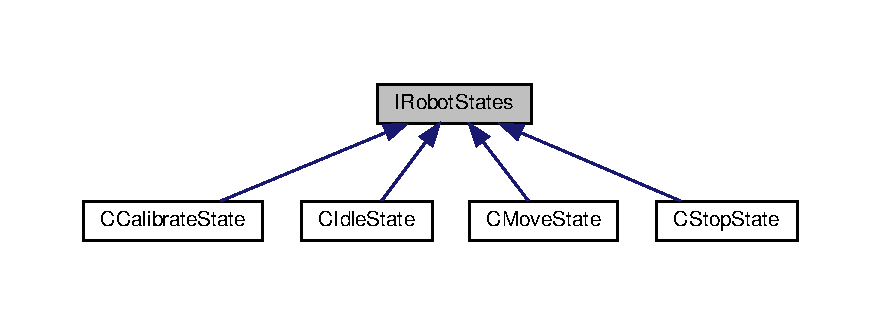
\includegraphics[width=350pt]{classIRobotStates__inherit__graph}
\end{center}
\end{figure}
\subsection*{Public Member Functions}
\begin{DoxyCompactItemize}
\item 
virtual void \hyperlink{classIRobotStates_af43ddb52f5100b42c3d11b71fb1f10dd}{Entry} ()=0
\begin{DoxyCompactList}\small\item\em the entry action which will be executed for the various states when the context enters that state. \end{DoxyCompactList}\item 
virtual void \hyperlink{classIRobotStates_aa681381e72738a2870c3f13f552a2e93}{Do} ()=0
\begin{DoxyCompactList}\small\item\em The do activity which will be executed after the entry action for the various states when the context enters that state. \end{DoxyCompactList}\item 
virtual void \hyperlink{classIRobotStates_a099417875e67f047ca38e08890491529}{Exit} ()=0
\begin{DoxyCompactList}\small\item\em The exit action which will executed when the context transitions off of the state. \end{DoxyCompactList}\item 
virtual void \hyperlink{classIRobotStates_a0b6c28a3deed04f93371a9395022f1ed}{Handle\+Event} (\hyperlink{classCEvent}{C\+Event} \&r\+Event, \hyperlink{classCRobotContext}{C\+Robot\+Context} \&r\+Context)=0
\begin{DoxyCompactList}\small\item\em The Handle\+Event function defines how the context will react to the next event, this depends on the state it is currently in. \end{DoxyCompactList}\end{DoxyCompactItemize}


\subsection{Member Function Documentation}
\mbox{\Hypertarget{classIRobotStates_aa681381e72738a2870c3f13f552a2e93}\label{classIRobotStates_aa681381e72738a2870c3f13f552a2e93}} 
\index{I\+Robot\+States@{I\+Robot\+States}!Do@{Do}}
\index{Do@{Do}!I\+Robot\+States@{I\+Robot\+States}}
\subsubsection{\texorpdfstring{Do()}{Do()}}
{\footnotesize\ttfamily virtual void I\+Robot\+States\+::\+Do (\begin{DoxyParamCaption}{ }\end{DoxyParamCaption})\hspace{0.3cm}{\ttfamily [pure virtual]}}



The do activity which will be executed after the entry action for the various states when the context enters that state. 



Implemented in \hyperlink{classCStopState_aba51445ef29e03fa5ffc5cef48923a10}{C\+Stop\+State}, \hyperlink{classCMoveState_acd364df1357b25ee616a7444116cf9f6}{C\+Move\+State}, \hyperlink{classCCalibrateState_a2b2ad369ae655704fadcffb0a4b9fca2}{C\+Calibrate\+State}, and \hyperlink{classCIdleState_a7ae1fe9a96dfb78faaebd068bb8ecae7}{C\+Idle\+State}.

\mbox{\Hypertarget{classIRobotStates_af43ddb52f5100b42c3d11b71fb1f10dd}\label{classIRobotStates_af43ddb52f5100b42c3d11b71fb1f10dd}} 
\index{I\+Robot\+States@{I\+Robot\+States}!Entry@{Entry}}
\index{Entry@{Entry}!I\+Robot\+States@{I\+Robot\+States}}
\subsubsection{\texorpdfstring{Entry()}{Entry()}}
{\footnotesize\ttfamily virtual void I\+Robot\+States\+::\+Entry (\begin{DoxyParamCaption}{ }\end{DoxyParamCaption})\hspace{0.3cm}{\ttfamily [pure virtual]}}



the entry action which will be executed for the various states when the context enters that state. 



Implemented in \hyperlink{classCStopState_aae7dbdb7db312f20a16fcd48edc60e83}{C\+Stop\+State}, \hyperlink{classCMoveState_ae9bda8d64d42c16e19facdfa8eb842e2}{C\+Move\+State}, \hyperlink{classCCalibrateState_a361368643bad182ed1a78ee1d1a820e5}{C\+Calibrate\+State}, and \hyperlink{classCIdleState_afcfc7e601c50b99c27380b9541fc3795}{C\+Idle\+State}.

\mbox{\Hypertarget{classIRobotStates_a099417875e67f047ca38e08890491529}\label{classIRobotStates_a099417875e67f047ca38e08890491529}} 
\index{I\+Robot\+States@{I\+Robot\+States}!Exit@{Exit}}
\index{Exit@{Exit}!I\+Robot\+States@{I\+Robot\+States}}
\subsubsection{\texorpdfstring{Exit()}{Exit()}}
{\footnotesize\ttfamily virtual void I\+Robot\+States\+::\+Exit (\begin{DoxyParamCaption}{ }\end{DoxyParamCaption})\hspace{0.3cm}{\ttfamily [pure virtual]}}



The exit action which will executed when the context transitions off of the state. 



Implemented in \hyperlink{classCStopState_a2bf7d1e44a9b0c689c86fb00f9684a7b}{C\+Stop\+State}, \hyperlink{classCMoveState_ac6f27ce9a561ab6baf297e106d3f346d}{C\+Move\+State}, \hyperlink{classCCalibrateState_a0bdb13da2af72f1e8e814a365f8d765a}{C\+Calibrate\+State}, and \hyperlink{classCIdleState_a634bf12d9a7f29504c7dc6df7d419835}{C\+Idle\+State}.

\mbox{\Hypertarget{classIRobotStates_a0b6c28a3deed04f93371a9395022f1ed}\label{classIRobotStates_a0b6c28a3deed04f93371a9395022f1ed}} 
\index{I\+Robot\+States@{I\+Robot\+States}!Handle\+Event@{Handle\+Event}}
\index{Handle\+Event@{Handle\+Event}!I\+Robot\+States@{I\+Robot\+States}}
\subsubsection{\texorpdfstring{Handle\+Event()}{HandleEvent()}}
{\footnotesize\ttfamily virtual void I\+Robot\+States\+::\+Handle\+Event (\begin{DoxyParamCaption}\item[{\hyperlink{classCEvent}{C\+Event} \&}]{r\+Event,  }\item[{\hyperlink{classCRobotContext}{C\+Robot\+Context} \&}]{r\+Context }\end{DoxyParamCaption})\hspace{0.3cm}{\ttfamily [pure virtual]}}



The Handle\+Event function defines how the context will react to the next event, this depends on the state it is currently in. 


\begin{DoxyParams}{Parameters}
{\em r\+Event} & The next event to be handle by the state machine \\
\hline
{\em r\+Context} & The context which will go through a state because of the incoming event. \\
\hline
\end{DoxyParams}


Implemented in \hyperlink{classCStopState_abe6af38d9c6b80b98fd78cdb48d7599c}{C\+Stop\+State}, \hyperlink{classCMoveState_a49c6051142c4839e1a512f38859589ad}{C\+Move\+State}, \hyperlink{classCCalibrateState_af24b30b6357a7b48f1157afdc0662984}{C\+Calibrate\+State}, and \hyperlink{classCIdleState_a12d0c6b590c56cdc9018524d632d4871}{C\+Idle\+State}.



The documentation for this class was generated from the following file\+:\begin{DoxyCompactItemize}
\item 
\hyperlink{IRobotStates_8h}{I\+Robot\+States.\+h}\end{DoxyCompactItemize}

\chapter{File Documentation}
\hypertarget{CEvent_8h}{}\section{C\+Event.\+h File Reference}
\label{CEvent_8h}\index{C\+Event.\+h@{C\+Event.\+h}}


The \hyperlink{classCEvent}{C\+Event} class is used as an event for the State machine, it holds instructions for servos and an eventtype to be used in the state machine.  


{\ttfamily \#include $<$vector$>$}\newline
{\ttfamily \#include $<$memory$>$}\newline
Include dependency graph for C\+Event.\+h\+:\nopagebreak
\begin{figure}[H]
\begin{center}
\leavevmode
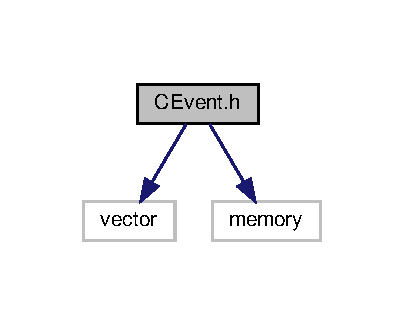
\includegraphics[width=194pt]{CEvent_8h__incl}
\end{center}
\end{figure}
This graph shows which files directly or indirectly include this file\+:\nopagebreak
\begin{figure}[H]
\begin{center}
\leavevmode
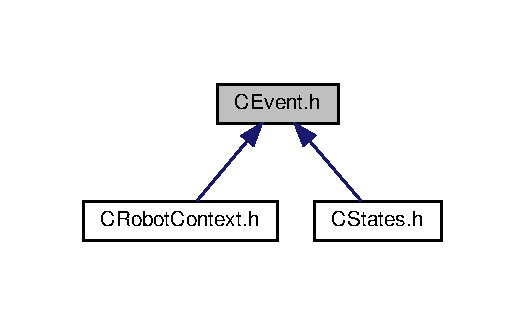
\includegraphics[width=252pt]{CEvent_8h__dep__incl}
\end{center}
\end{figure}
\subsection*{Classes}
\begin{DoxyCompactItemize}
\item 
class \hyperlink{classCEvent}{C\+Event}
\end{DoxyCompactItemize}
\subsection*{Enumerations}
\begin{DoxyCompactItemize}
\item 
\mbox{\Hypertarget{CEvent_8h_a052e637824ed8cb8a5e9d5d73b5b3c8b}\label{CEvent_8h_a052e637824ed8cb8a5e9d5d73b5b3c8b}} 
enum {\bfseries e\+Event\+Type} \{ {\bfseries I\+D\+LE}, 
{\bfseries M\+O\+VE}, 
{\bfseries C\+A\+L\+I\+B\+R\+A\+TE}, 
{\bfseries E\+M\+E\+R\+G\+E\+N\+C\+Y\+\_\+\+S\+T\+OP}
 \}
\end{DoxyCompactItemize}


\subsection{Detailed Description}
The \hyperlink{classCEvent}{C\+Event} class is used as an event for the State machine, it holds instructions for servos and an eventtype to be used in the state machine. 

\begin{DoxyAuthor}{Author}
Evren Kilic (\href{mailto:ET.Kilic@student.han.nl}{\tt E\+T.\+Kilic@student.\+han.\+nl}) 
\end{DoxyAuthor}
\begin{DoxyVersion}{Version}
0.\+1 
\end{DoxyVersion}
\begin{DoxyDate}{Date}
11-\/03-\/2020
\end{DoxyDate}
\begin{DoxyCopyright}{Copyright}
Copyright (c) 2020 
\end{DoxyCopyright}

\hypertarget{CRobotContext_8h}{}\section{C\+Robot\+Context.\+h File Reference}
\label{CRobotContext_8h}\index{C\+Robot\+Context.\+h@{C\+Robot\+Context.\+h}}


The \hyperlink{classCRobotContext}{C\+Robot\+Context} is the context for the state machine which controlls the robot arm through its states of moving, idling, calibrating, and stopping. It also holds a nodehandle with which it subscribes to ros topics on which instructions get published.  


{\ttfamily \#include $<$ros/ros.\+h$>$}\newline
{\ttfamily \#include $<$memory$>$}\newline
{\ttfamily \#include $<$queue$>$}\newline
{\ttfamily \#include $<$chrono$>$}\newline
{\ttfamily \#include \char`\"{}C\+Event.\+h\char`\"{}}\newline
{\ttfamily \#include \char`\"{}Robot\+Arm\+Controller/\+Move.\+h\char`\"{}}\newline
{\ttfamily \#include \char`\"{}Robot\+Arm\+Controller/\+Emergency\+Stop.\+h\char`\"{}}\newline
{\ttfamily \#include \char`\"{}Robot\+Arm\+Controller/\+Programmed\+Position.\+h\char`\"{}}\newline
Include dependency graph for C\+Robot\+Context.\+h\+:\nopagebreak
\begin{figure}[H]
\begin{center}
\leavevmode
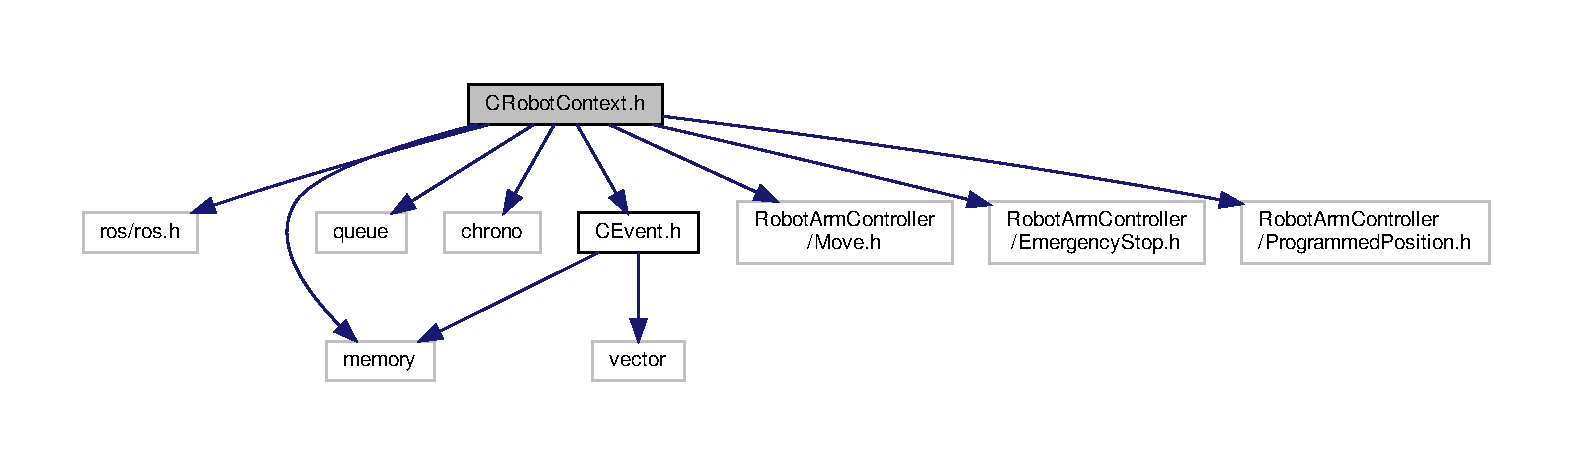
\includegraphics[width=350pt]{CRobotContext_8h__incl}
\end{center}
\end{figure}
\subsection*{Classes}
\begin{DoxyCompactItemize}
\item 
class \hyperlink{classCRobotContext}{C\+Robot\+Context}
\end{DoxyCompactItemize}


\subsection{Detailed Description}
The \hyperlink{classCRobotContext}{C\+Robot\+Context} is the context for the state machine which controlls the robot arm through its states of moving, idling, calibrating, and stopping. It also holds a nodehandle with which it subscribes to ros topics on which instructions get published. 

\begin{DoxyAuthor}{Author}
Evren Kilic (\href{mailto:ET.Kilic@student.han.nl}{\tt E\+T.\+Kilic@student.\+han.\+nl}) 
\end{DoxyAuthor}
\begin{DoxyVersion}{Version}
0.\+1 
\end{DoxyVersion}
\begin{DoxyDate}{Date}
05-\/03-\/2020
\end{DoxyDate}
\begin{DoxyCopyright}{Copyright}
Copyright (c) 2020 
\end{DoxyCopyright}

\hypertarget{CServoInstruction_8h}{}\section{C\+Servo\+Instruction.\+h File Reference}
\label{CServoInstruction_8h}\index{C\+Servo\+Instruction.\+h@{C\+Servo\+Instruction.\+h}}


C\+Servoinstruction is a class that holds the instructions for a specfic servo within the robotarm.  


{\ttfamily \#include $<$stdint.\+h$>$}\newline
{\ttfamily \#include \char`\"{}Robot\+High\+Level/\+C\+Configuration.\+h\char`\"{}}\newline
Include dependency graph for C\+Servo\+Instruction.\+h\+:\nopagebreak
\begin{figure}[H]
\begin{center}
\leavevmode
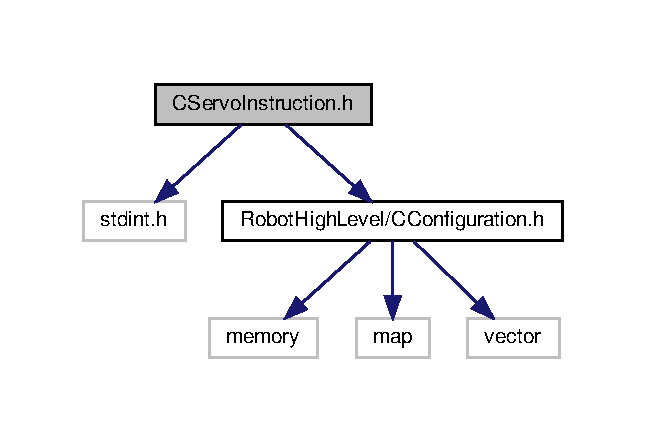
\includegraphics[width=310pt]{CServoInstruction_8h__incl}
\end{center}
\end{figure}
This graph shows which files directly or indirectly include this file\+:\nopagebreak
\begin{figure}[H]
\begin{center}
\leavevmode
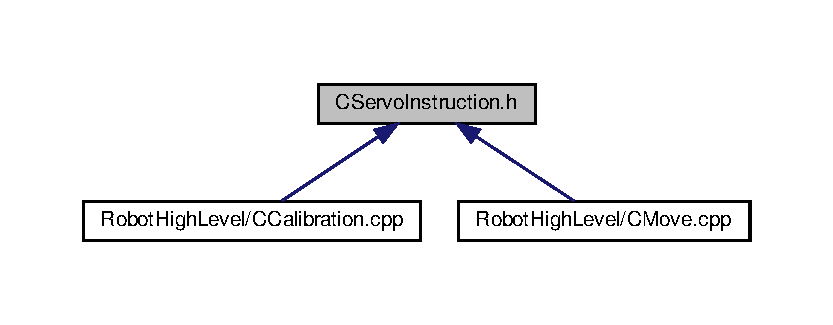
\includegraphics[width=350pt]{CServoInstruction_8h__dep__incl}
\end{center}
\end{figure}
\subsection*{Classes}
\begin{DoxyCompactItemize}
\item 
class \hyperlink{classCServoInstruction}{C\+Servo\+Instruction}
\end{DoxyCompactItemize}


\subsection{Detailed Description}
C\+Servoinstruction is a class that holds the instructions for a specfic servo within the robotarm. 

\begin{DoxyAuthor}{Author}
Evren Kilic (\href{mailto:ET.Kilic@student.han.nl}{\tt E\+T.\+Kilic@student.\+han.\+nl}) 
\end{DoxyAuthor}
\begin{DoxyVersion}{Version}
0.\+1 
\end{DoxyVersion}
\begin{DoxyDate}{Date}
11-\/03-\/2020
\end{DoxyDate}
\begin{DoxyCopyright}{Copyright}
Copyright (c) 2020 
\end{DoxyCopyright}

\hypertarget{CStatePublisher_8h}{}\section{C\+State\+Publisher.\+h File Reference}
\label{CStatePublisher_8h}\index{C\+State\+Publisher.\+h@{C\+State\+Publisher.\+h}}


\hyperlink{classCStatePublisher}{C\+State\+Publisher} is a singleton class that can be used to publish a state on the /\+Robot\+Arm\+Controller/\+State ros topic.  


{\ttfamily \#include $<$ros/ros.\+h$>$}\newline
Include dependency graph for C\+State\+Publisher.\+h\+:\nopagebreak
\begin{figure}[H]
\begin{center}
\leavevmode
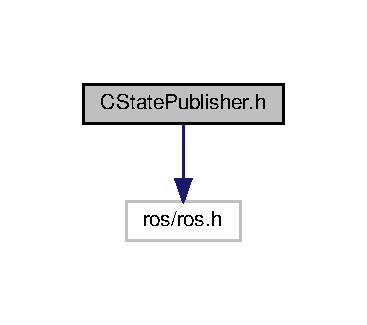
\includegraphics[width=176pt]{CStatePublisher_8h__incl}
\end{center}
\end{figure}
\subsection*{Classes}
\begin{DoxyCompactItemize}
\item 
class \hyperlink{classCStatePublisher}{C\+State\+Publisher}
\end{DoxyCompactItemize}
\subsection*{Enumerations}
\begin{DoxyCompactItemize}
\item 
enum \hyperlink{CStatePublisher_8h_a57ce604a7850ac5988b6182daf162fe9}{e\+Publishable\+States} \{ {\bfseries P\+U\+B\+L\+I\+S\+H\+\_\+\+I\+D\+LE}, 
{\bfseries P\+U\+B\+L\+I\+S\+H\+\_\+\+M\+O\+VE}, 
{\bfseries P\+U\+B\+L\+I\+S\+H\+\_\+\+C\+A\+L\+I\+B\+R\+A\+TE}, 
{\bfseries P\+U\+B\+L\+I\+S\+H\+\_\+\+E\+M\+E\+R\+G\+E\+N\+C\+Y\+\_\+\+S\+T\+OP}
 \}\begin{DoxyCompactList}\small\item\em The enum of states that the state publisher can publish. \end{DoxyCompactList}
\end{DoxyCompactItemize}


\subsection{Detailed Description}
\hyperlink{classCStatePublisher}{C\+State\+Publisher} is a singleton class that can be used to publish a state on the /\+Robot\+Arm\+Controller/\+State ros topic. 

\begin{DoxyAuthor}{Author}
Evren Kilic (\href{mailto:ET.Kilic@student.han.nl}{\tt E\+T.\+Kilic@student.\+han.\+nl}) 
\end{DoxyAuthor}
\begin{DoxyVersion}{Version}
0.\+1 
\end{DoxyVersion}
\begin{DoxyDate}{Date}
05-\/03-\/2020
\end{DoxyDate}
\begin{DoxyCopyright}{Copyright}
Copyright (c) 2020 
\end{DoxyCopyright}


\subsection{Enumeration Type Documentation}
\mbox{\Hypertarget{CStatePublisher_8h_a57ce604a7850ac5988b6182daf162fe9}\label{CStatePublisher_8h_a57ce604a7850ac5988b6182daf162fe9}} 
\index{C\+State\+Publisher.\+h@{C\+State\+Publisher.\+h}!e\+Publishable\+States@{e\+Publishable\+States}}
\index{e\+Publishable\+States@{e\+Publishable\+States}!C\+State\+Publisher.\+h@{C\+State\+Publisher.\+h}}
\subsubsection{\texorpdfstring{e\+Publishable\+States}{ePublishableStates}}
{\footnotesize\ttfamily enum \hyperlink{CStatePublisher_8h_a57ce604a7850ac5988b6182daf162fe9}{e\+Publishable\+States}}



The enum of states that the state publisher can publish. 


\hypertarget{CStates_8h}{}\section{C\+States.\+h File Reference}
\label{CStates_8h}\index{C\+States.\+h@{C\+States.\+h}}


In this file are the various states which the Robot\+Arm\+Controller\textquotesingle{}s state machine can be in.  


{\ttfamily \#include \char`\"{}C\+Event.\+h\char`\"{}}\newline
{\ttfamily \#include \char`\"{}I\+Robot\+States.\+h\char`\"{}}\newline
{\ttfamily \#include $<$memory$>$}\newline
Include dependency graph for C\+States.\+h\+:\nopagebreak
\begin{figure}[H]
\begin{center}
\leavevmode
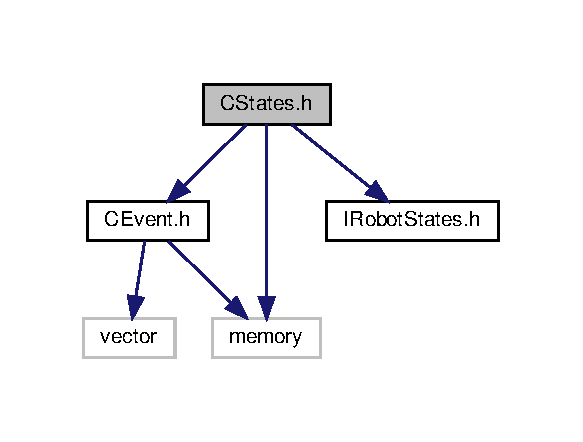
\includegraphics[width=280pt]{CStates_8h__incl}
\end{center}
\end{figure}
\subsection*{Classes}
\begin{DoxyCompactItemize}
\item 
class \hyperlink{classCIdleState}{C\+Idle\+State}
\item 
class \hyperlink{classCCalibrateState}{C\+Calibrate\+State}
\item 
class \hyperlink{classCMoveState}{C\+Move\+State}
\item 
class \hyperlink{classCStopState}{C\+Stop\+State}
\end{DoxyCompactItemize}


\subsection{Detailed Description}
In this file are the various states which the Robot\+Arm\+Controller\textquotesingle{}s state machine can be in. 

\begin{DoxyAuthor}{Author}
Evren Kilic (\href{mailto:ET.Kilic@student.han.nl}{\tt E\+T.\+Kilic@student.\+han.\+nl}) 
\end{DoxyAuthor}
\begin{DoxyVersion}{Version}
0.\+1 
\end{DoxyVersion}
\begin{DoxyDate}{Date}
11-\/03-\/2020
\end{DoxyDate}
\begin{DoxyCopyright}{Copyright}
Copyright (c) 2020 
\end{DoxyCopyright}

\hypertarget{IRobotStates_8h}{}\section{I\+Robot\+States.\+h File Reference}
\label{IRobotStates_8h}\index{I\+Robot\+States.\+h@{I\+Robot\+States.\+h}}


The interface for the various classes in the state machine.  


This graph shows which files directly or indirectly include this file\+:\nopagebreak
\begin{figure}[H]
\begin{center}
\leavevmode
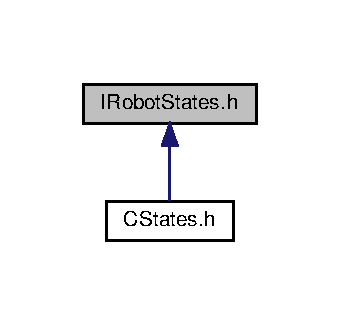
\includegraphics[width=163pt]{IRobotStates_8h__dep__incl}
\end{center}
\end{figure}
\subsection*{Classes}
\begin{DoxyCompactItemize}
\item 
class \hyperlink{classIRobotStates}{I\+Robot\+States}
\end{DoxyCompactItemize}


\subsection{Detailed Description}
The interface for the various classes in the state machine. 

\begin{DoxyAuthor}{Author}
Evren Kilic (\href{mailto:ET.Kilic@student.han.nl}{\tt E\+T.\+Kilic@student.\+han.\+nl}) 
\end{DoxyAuthor}
\begin{DoxyVersion}{Version}
0.\+1 
\end{DoxyVersion}
\begin{DoxyDate}{Date}
11-\/03-\/2020
\end{DoxyDate}
\begin{DoxyCopyright}{Copyright}
Copyright (c) 2020 
\end{DoxyCopyright}

\hypertarget{CCalibration_8cpp}{}\section{Robot\+High\+Level/\+C\+Calibration.cpp File Reference}
\label{CCalibration_8cpp}\index{Robot\+High\+Level/\+C\+Calibration.\+cpp@{Robot\+High\+Level/\+C\+Calibration.\+cpp}}
{\ttfamily \#include \char`\"{}C\+Calibration.\+h\char`\"{}}\newline
{\ttfamily \#include \char`\"{}../\+C\+Servo\+Instruction.\+h\char`\"{}}\newline
{\ttfamily \#include \char`\"{}C\+Move.\+h\char`\"{}}\newline
Include dependency graph for C\+Calibration.\+cpp\+:\nopagebreak
\begin{figure}[H]
\begin{center}
\leavevmode
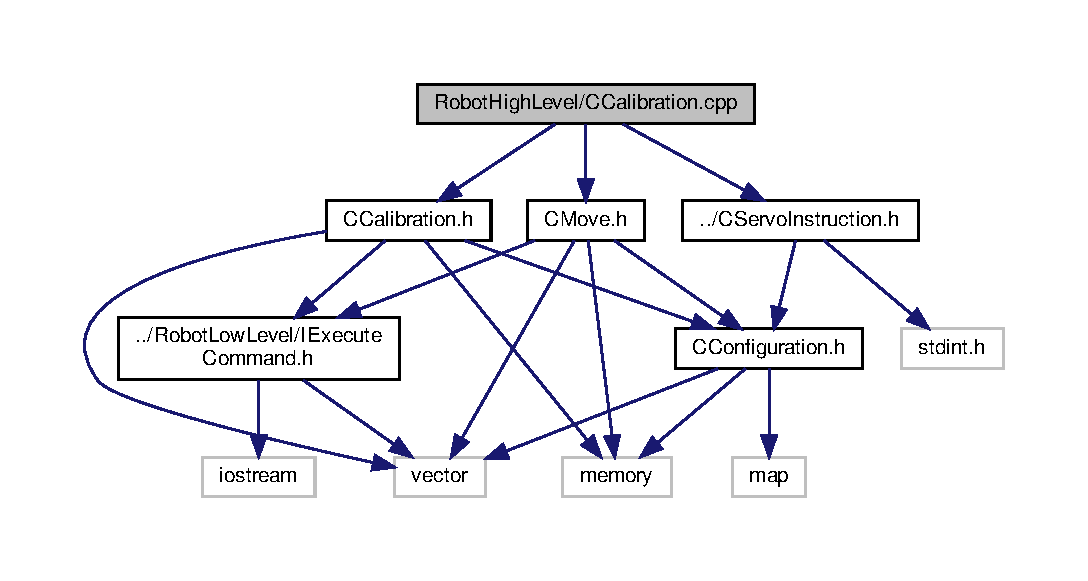
\includegraphics[width=350pt]{CCalibration_8cpp__incl}
\end{center}
\end{figure}


\subsection{Detailed Description}
\begin{DoxyAuthor}{Author}
Tim Beeren (\href{mailto:T.Beeren1@student.han.nl}{\tt T.\+Beeren1@student.\+han.\+nl}) 
\end{DoxyAuthor}
\begin{DoxyVersion}{Version}
0.\+1 
\end{DoxyVersion}
\begin{DoxyDate}{Date}
06-\/03-\/2020
\end{DoxyDate}
\begin{DoxyCopyright}{Copyright}
Copyright (c) 2020 
\end{DoxyCopyright}

\hypertarget{CCalibration_8h}{}\section{Robot\+High\+Level/\+C\+Calibration.h File Reference}
\label{CCalibration_8h}\index{Robot\+High\+Level/\+C\+Calibration.\+h@{Robot\+High\+Level/\+C\+Calibration.\+h}}


The Calibration class is responsible for handling calibrations for the servo boundries.  


{\ttfamily \#include $<$memory$>$}\newline
{\ttfamily \#include $<$vector$>$}\newline
{\ttfamily \#include \char`\"{}C\+Configuration.\+h\char`\"{}}\newline
{\ttfamily \#include \char`\"{}../\+Robot\+Low\+Level/\+I\+Execute\+Command.\+h\char`\"{}}\newline
Include dependency graph for C\+Calibration.\+h\+:\nopagebreak
\begin{figure}[H]
\begin{center}
\leavevmode
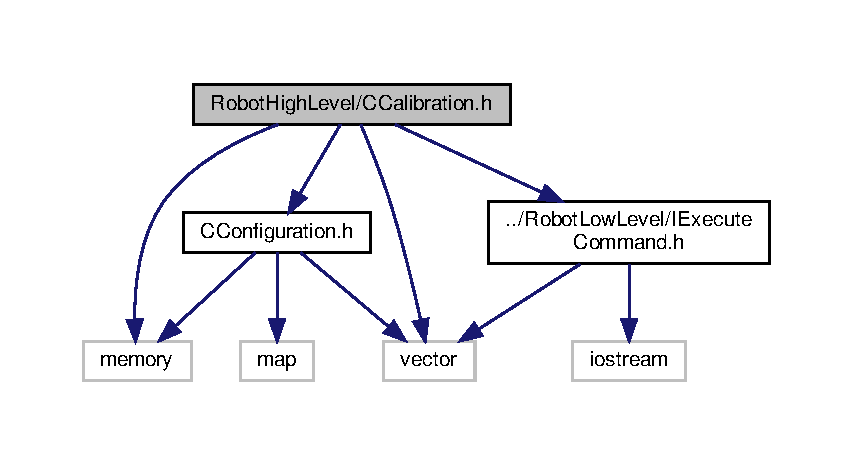
\includegraphics[width=350pt]{CCalibration_8h__incl}
\end{center}
\end{figure}
This graph shows which files directly or indirectly include this file\+:\nopagebreak
\begin{figure}[H]
\begin{center}
\leavevmode
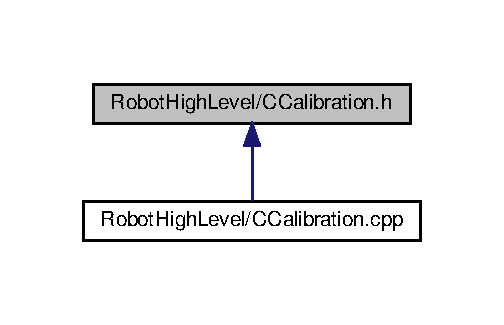
\includegraphics[width=242pt]{CCalibration_8h__dep__incl}
\end{center}
\end{figure}
\subsection*{Classes}
\begin{DoxyCompactItemize}
\item 
class \hyperlink{classCCalibration}{C\+Calibration}
\end{DoxyCompactItemize}


\subsection{Detailed Description}
The Calibration class is responsible for handling calibrations for the servo boundries. 

\begin{DoxyAuthor}{Author}
Tim Beeren (\href{mailto:T.Beeren1@student.han.nl}{\tt T.\+Beeren1@student.\+han.\+nl}) 
\end{DoxyAuthor}
\begin{DoxyVersion}{Version}
0.\+1 
\end{DoxyVersion}
\begin{DoxyDate}{Date}
06-\/03-\/2020
\end{DoxyDate}
\begin{DoxyCopyright}{Copyright}
Copyright (c) 2020 
\end{DoxyCopyright}

\hypertarget{CConfiguration_8cpp}{}\section{Robot\+High\+Level/\+C\+Configuration.cpp File Reference}
\label{CConfiguration_8cpp}\index{Robot\+High\+Level/\+C\+Configuration.\+cpp@{Robot\+High\+Level/\+C\+Configuration.\+cpp}}
{\ttfamily \#include \char`\"{}C\+Configuration.\+h\char`\"{}}\newline
{\ttfamily \#include $<$iostream$>$}\newline
Include dependency graph for C\+Configuration.\+cpp\+:\nopagebreak
\begin{figure}[H]
\begin{center}
\leavevmode
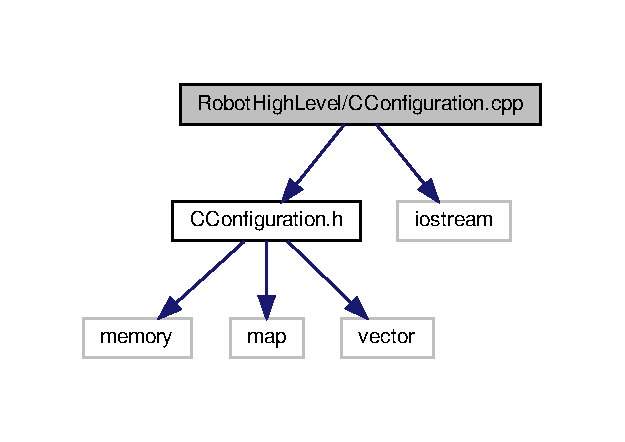
\includegraphics[width=300pt]{CConfiguration_8cpp__incl}
\end{center}
\end{figure}


\subsection{Detailed Description}
\begin{DoxyAuthor}{Author}
Tim Beeren (\href{mailto:T.Beeren1@student.han.nl}{\tt T.\+Beeren1@student.\+han.\+nl}) 
\end{DoxyAuthor}
\begin{DoxyVersion}{Version}
0.\+1 
\end{DoxyVersion}
\begin{DoxyDate}{Date}
06-\/03-\/2020
\end{DoxyDate}
\begin{DoxyCopyright}{Copyright}
Copyright (c) 2020 
\end{DoxyCopyright}

\hypertarget{CConfiguration_8h}{}\section{Robot\+High\+Level/\+C\+Configuration.h File Reference}
\label{CConfiguration_8h}\index{Robot\+High\+Level/\+C\+Configuration.\+h@{Robot\+High\+Level/\+C\+Configuration.\+h}}


The configuration class holds the calibrated values for every servo.  


{\ttfamily \#include $<$memory$>$}\newline
{\ttfamily \#include $<$map$>$}\newline
{\ttfamily \#include $<$vector$>$}\newline
Include dependency graph for C\+Configuration.\+h\+:\nopagebreak
\begin{figure}[H]
\begin{center}
\leavevmode
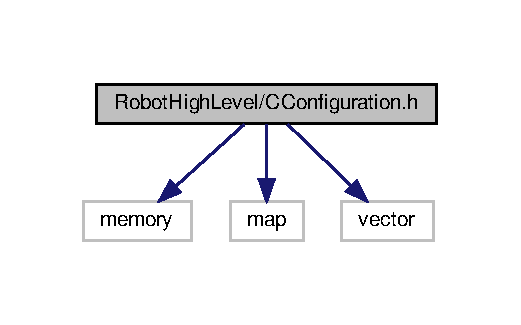
\includegraphics[width=250pt]{CConfiguration_8h__incl}
\end{center}
\end{figure}
This graph shows which files directly or indirectly include this file\+:\nopagebreak
\begin{figure}[H]
\begin{center}
\leavevmode
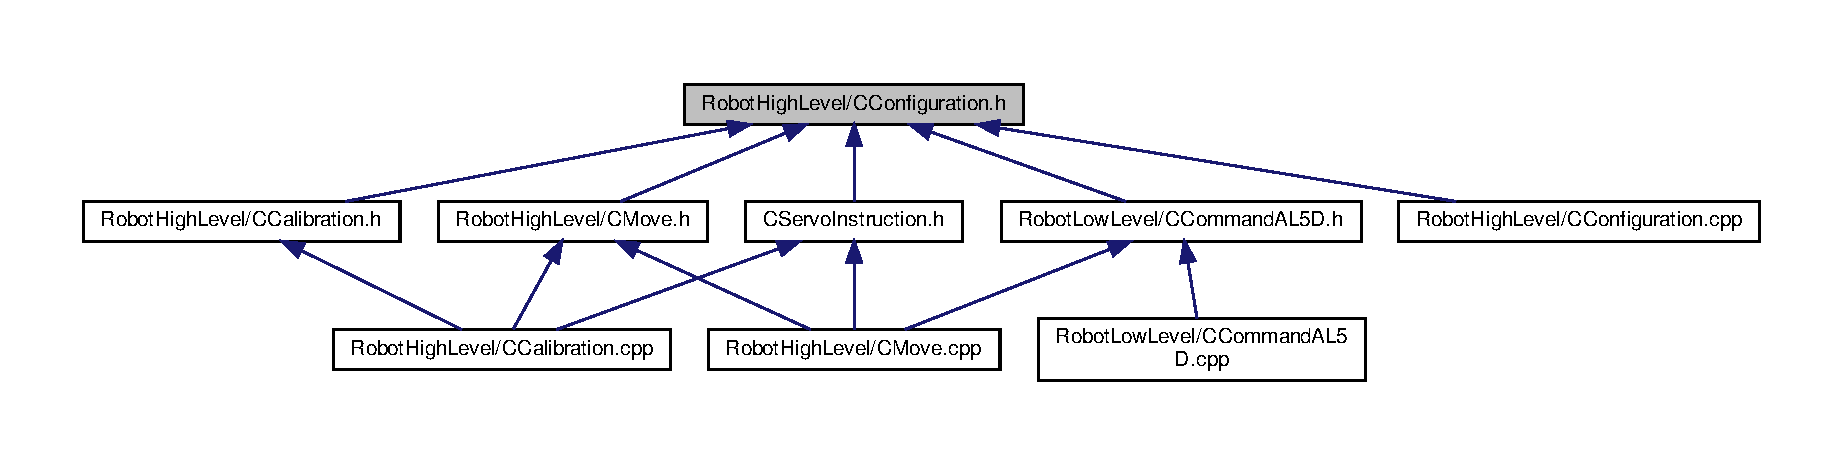
\includegraphics[width=350pt]{CConfiguration_8h__dep__incl}
\end{center}
\end{figure}
\subsection*{Classes}
\begin{DoxyCompactItemize}
\item 
class \hyperlink{classCConfiguration}{C\+Configuration}
\end{DoxyCompactItemize}
\subsection*{Enumerations}
\begin{DoxyCompactItemize}
\item 
\mbox{\Hypertarget{CConfiguration_8h_a4b59ba106ee17cbd0cf85f56b583f5b0}\label{CConfiguration_8h_a4b59ba106ee17cbd0cf85f56b583f5b0}} 
enum {\bfseries e\+Servos} \{ \newline
{\bfseries B\+A\+SE} = 0, 
{\bfseries S\+H\+O\+U\+L\+D\+ER} = 1, 
{\bfseries E\+L\+B\+OW} = 2, 
{\bfseries W\+R\+I\+ST} = 3, 
\newline
{\bfseries G\+R\+I\+P\+P\+ER} = 4, 
{\bfseries W\+R\+I\+S\+T\+\_\+\+R\+O\+T\+A\+TE} = 5, 
{\bfseries U\+N\+K\+N\+O\+W\+N\+\_\+\+S\+E\+R\+VO} = 6
 \}
\item 
\mbox{\Hypertarget{CConfiguration_8h_adb7b2b138da65199b8a846dff2e5c7aa}\label{CConfiguration_8h_adb7b2b138da65199b8a846dff2e5c7aa}} 
enum {\bfseries e\+Programmed\+Position} \{ {\bfseries P\+A\+RK}, 
{\bfseries R\+E\+A\+DY}, 
{\bfseries S\+T\+R\+A\+I\+G\+HT}
 \}
\end{DoxyCompactItemize}


\subsection{Detailed Description}
The configuration class holds the calibrated values for every servo. 

\begin{DoxyAuthor}{Author}
Tim Beeren (\href{mailto:T.Beeren1@student.han.nl}{\tt T.\+Beeren1@student.\+han.\+nl}) 
\end{DoxyAuthor}
\begin{DoxyVersion}{Version}
0.\+1 
\end{DoxyVersion}
\begin{DoxyDate}{Date}
06-\/03-\/2020
\end{DoxyDate}
\begin{DoxyCopyright}{Copyright}
Copyright (c) 2020 
\end{DoxyCopyright}

\hypertarget{CMove_8cpp}{}\section{Robot\+High\+Level/\+C\+Move.cpp File Reference}
\label{CMove_8cpp}\index{Robot\+High\+Level/\+C\+Move.\+cpp@{Robot\+High\+Level/\+C\+Move.\+cpp}}
{\ttfamily \#include \char`\"{}C\+Move.\+h\char`\"{}}\newline
{\ttfamily \#include \char`\"{}../\+C\+Servo\+Instruction.\+h\char`\"{}}\newline
{\ttfamily \#include \char`\"{}../\+Robot\+Low\+Level/\+C\+Command\+A\+L5\+D.\+h\char`\"{}}\newline
{\ttfamily \#include $<$assert.\+h$>$}\newline
Include dependency graph for C\+Move.\+cpp\+:\nopagebreak
\begin{figure}[H]
\begin{center}
\leavevmode
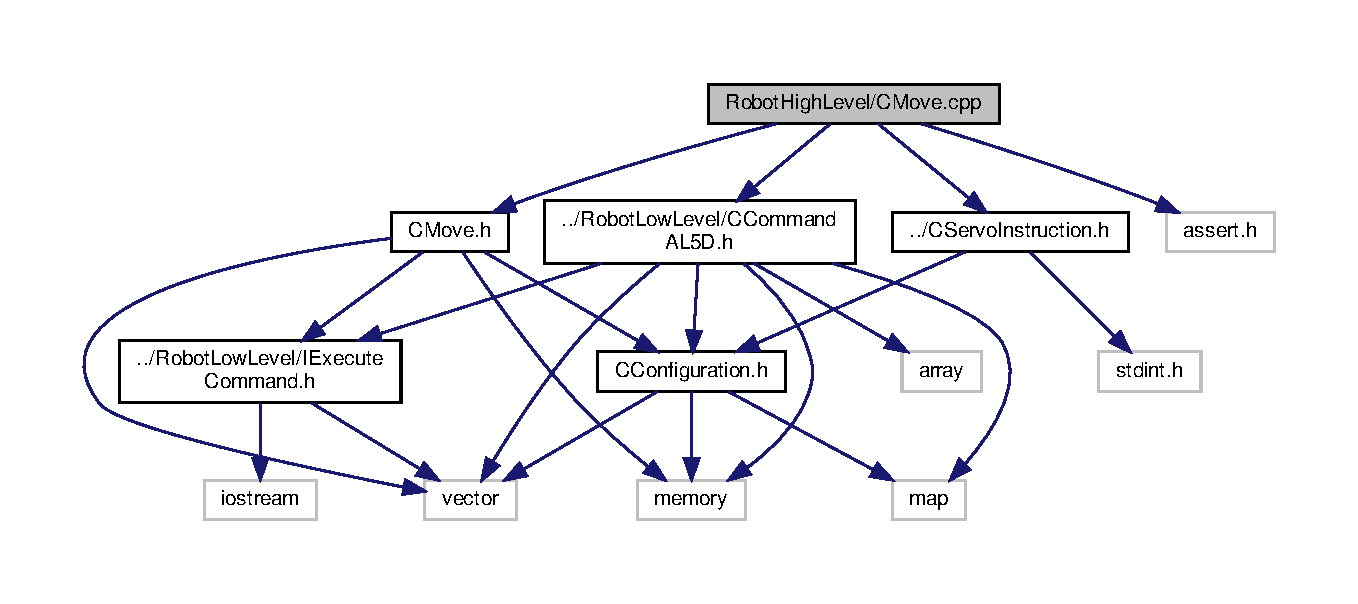
\includegraphics[width=350pt]{CMove_8cpp__incl}
\end{center}
\end{figure}


\subsection{Detailed Description}
\begin{DoxyAuthor}{Author}
Tim Beeren (\href{mailto:T.Beeren1@student.han.nl}{\tt T.\+Beeren1@student.\+han.\+nl}) 
\end{DoxyAuthor}
\begin{DoxyVersion}{Version}
0.\+1 
\end{DoxyVersion}
\begin{DoxyDate}{Date}
06-\/03-\/2020
\end{DoxyDate}
\begin{DoxyCopyright}{Copyright}
Copyright (c) 2020 
\end{DoxyCopyright}

\hypertarget{CMove_8h}{}\section{Robot\+High\+Level/\+C\+Move.h File Reference}
\label{CMove_8h}\index{Robot\+High\+Level/\+C\+Move.\+h@{Robot\+High\+Level/\+C\+Move.\+h}}


The \hyperlink{classCMove}{C\+Move} class offers functions to calculate degrees to P\+WM and to then send a command to the robotarm that will make it move.  


{\ttfamily \#include $<$vector$>$}\newline
{\ttfamily \#include $<$memory$>$}\newline
{\ttfamily \#include \char`\"{}../\+Robot\+Low\+Level/\+I\+Execute\+Command.\+h\char`\"{}}\newline
{\ttfamily \#include \char`\"{}C\+Configuration.\+h\char`\"{}}\newline
Include dependency graph for C\+Move.\+h\+:\nopagebreak
\begin{figure}[H]
\begin{center}
\leavevmode
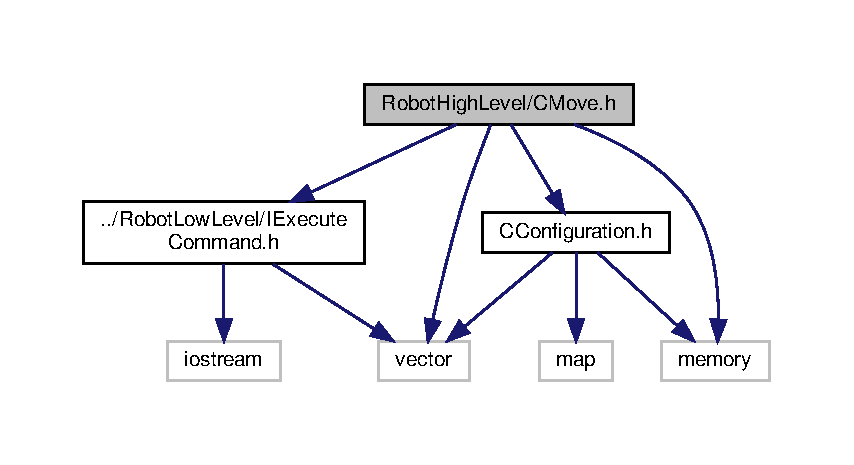
\includegraphics[width=350pt]{CMove_8h__incl}
\end{center}
\end{figure}
This graph shows which files directly or indirectly include this file\+:\nopagebreak
\begin{figure}[H]
\begin{center}
\leavevmode
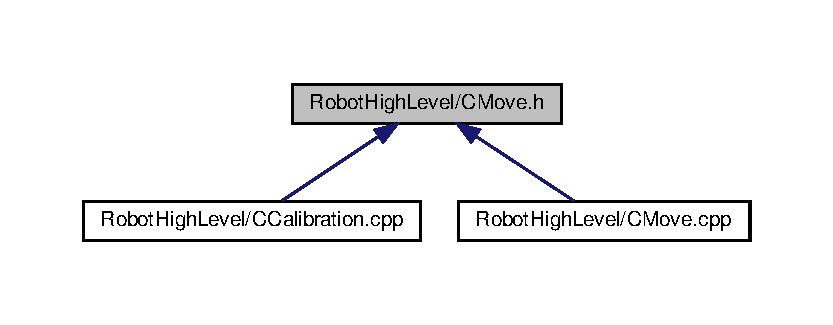
\includegraphics[width=350pt]{CMove_8h__dep__incl}
\end{center}
\end{figure}
\subsection*{Classes}
\begin{DoxyCompactItemize}
\item 
class \hyperlink{classCMove}{C\+Move}
\end{DoxyCompactItemize}


\subsection{Detailed Description}
The \hyperlink{classCMove}{C\+Move} class offers functions to calculate degrees to P\+WM and to then send a command to the robotarm that will make it move. 

\begin{DoxyAuthor}{Author}
Tim Beeren (\href{mailto:T.Beeren1@student.han.nl}{\tt T.\+Beeren1@student.\+han.\+nl}) 
\end{DoxyAuthor}
\begin{DoxyVersion}{Version}
0.\+1 
\end{DoxyVersion}
\begin{DoxyDate}{Date}
12-\/03-\/2020
\end{DoxyDate}
\begin{DoxyCopyright}{Copyright}
Copyright (c) 2020 
\end{DoxyCopyright}

\hypertarget{CCommandAL5D_8cpp}{}\section{Robot\+Low\+Level/\+C\+Command\+A\+L5D.cpp File Reference}
\label{CCommandAL5D_8cpp}\index{Robot\+Low\+Level/\+C\+Command\+A\+L5\+D.\+cpp@{Robot\+Low\+Level/\+C\+Command\+A\+L5\+D.\+cpp}}
{\ttfamily \#include \char`\"{}C\+Command\+A\+L5\+D.\+h\char`\"{}}\newline
{\ttfamily \#include \char`\"{}C\+Communicate.\+h\char`\"{}}\newline
Include dependency graph for C\+Command\+A\+L5\+D.\+cpp\+:\nopagebreak
\begin{figure}[H]
\begin{center}
\leavevmode
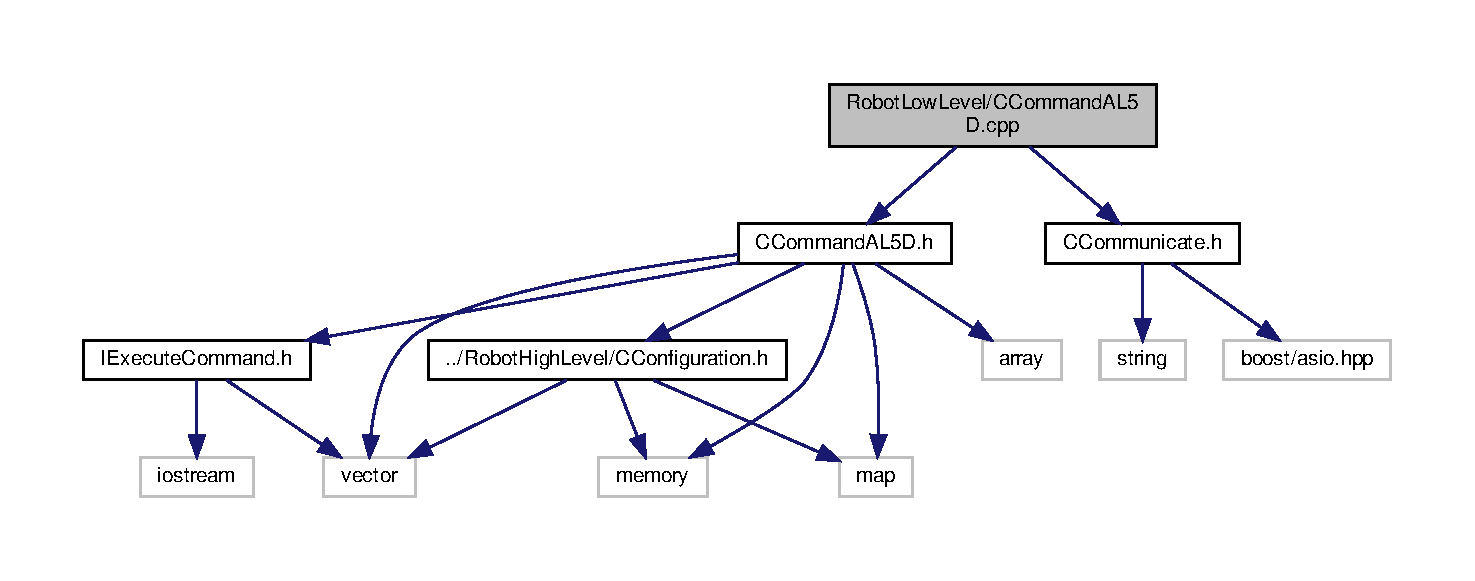
\includegraphics[width=350pt]{CCommandAL5D_8cpp__incl}
\end{center}
\end{figure}


\subsection{Detailed Description}
\begin{DoxyAuthor}{Author}
Tim Beeren (\href{mailto:T.Beeren1@student.han.nl}{\tt T.\+Beeren1@student.\+han.\+nl}) 
\end{DoxyAuthor}
\begin{DoxyVersion}{Version}
0.\+1 
\end{DoxyVersion}
\begin{DoxyDate}{Date}
06-\/03-\/2020
\end{DoxyDate}
\begin{DoxyCopyright}{Copyright}
Copyright (c) 2020 
\end{DoxyCopyright}

\hypertarget{CCommandAL5D_8h}{}\section{Robot\+Low\+Level/\+C\+Command\+A\+L5D.h File Reference}
\label{CCommandAL5D_8h}\index{Robot\+Low\+Level/\+C\+Command\+A\+L5\+D.\+h@{Robot\+Low\+Level/\+C\+Command\+A\+L5\+D.\+h}}


The Command\+A\+L5D class is a realistation of the \hyperlink{classIExecuteCommand}{I\+Execute\+Command}. It is reponsible for commanding the A\+L5D robotarm and is used by higher level drivers.  


{\ttfamily \#include \char`\"{}I\+Execute\+Command.\+h\char`\"{}}\newline
{\ttfamily \#include \char`\"{}../\+Robot\+High\+Level/\+C\+Configuration.\+h\char`\"{}}\newline
{\ttfamily \#include $<$memory$>$}\newline
{\ttfamily \#include $<$vector$>$}\newline
{\ttfamily \#include $<$map$>$}\newline
{\ttfamily \#include $<$array$>$}\newline
Include dependency graph for C\+Command\+A\+L5\+D.\+h\+:\nopagebreak
\begin{figure}[H]
\begin{center}
\leavevmode
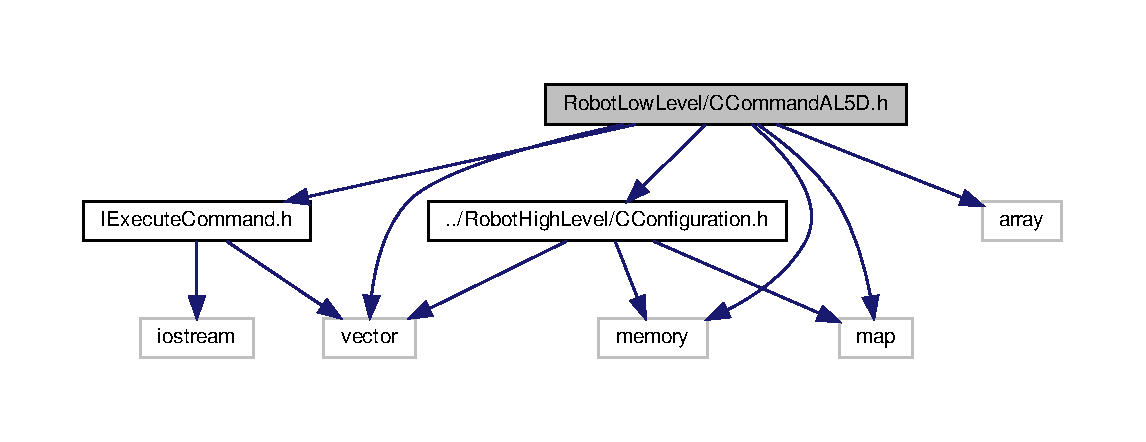
\includegraphics[width=350pt]{CCommandAL5D_8h__incl}
\end{center}
\end{figure}
This graph shows which files directly or indirectly include this file\+:\nopagebreak
\begin{figure}[H]
\begin{center}
\leavevmode
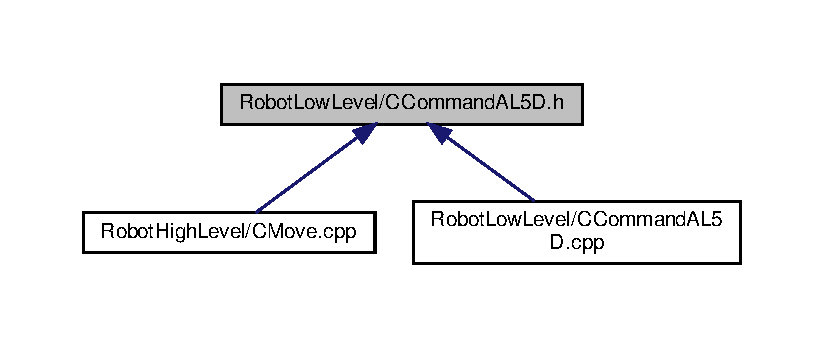
\includegraphics[width=350pt]{CCommandAL5D_8h__dep__incl}
\end{center}
\end{figure}
\subsection*{Classes}
\begin{DoxyCompactItemize}
\item 
class \hyperlink{classCCommandAL5D}{C\+Command\+A\+L5D}
\end{DoxyCompactItemize}


\subsection{Detailed Description}
The Command\+A\+L5D class is a realistation of the \hyperlink{classIExecuteCommand}{I\+Execute\+Command}. It is reponsible for commanding the A\+L5D robotarm and is used by higher level drivers. 

\begin{DoxyAuthor}{Author}
Tim Beeren (\href{mailto:T.Beeren1@student.han.nl}{\tt T.\+Beeren1@student.\+han.\+nl}) 
\end{DoxyAuthor}
\begin{DoxyVersion}{Version}
0.\+1 
\end{DoxyVersion}
\begin{DoxyDate}{Date}
06-\/03-\/2020
\end{DoxyDate}
\begin{DoxyCopyright}{Copyright}
Copyright (c) 2020 
\end{DoxyCopyright}

\hypertarget{CCommunicate_8cpp}{}\section{Robot\+Low\+Level/\+C\+Communicate.cpp File Reference}
\label{CCommunicate_8cpp}\index{Robot\+Low\+Level/\+C\+Communicate.\+cpp@{Robot\+Low\+Level/\+C\+Communicate.\+cpp}}
{\ttfamily \#include \char`\"{}C\+Communicate.\+h\char`\"{}}\newline
{\ttfamily \#include $<$iostream$>$}\newline
Include dependency graph for C\+Communicate.\+cpp\+:\nopagebreak
\begin{figure}[H]
\begin{center}
\leavevmode
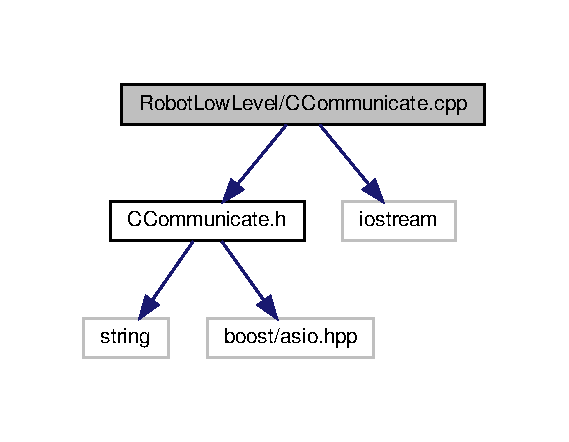
\includegraphics[width=273pt]{CCommunicate_8cpp__incl}
\end{center}
\end{figure}


\subsection{Detailed Description}
\begin{DoxyAuthor}{Author}
Tim Beeren (\href{mailto:T.Beeren1@student.han.nl}{\tt T.\+Beeren1@student.\+han.\+nl}) 
\end{DoxyAuthor}
\begin{DoxyVersion}{Version}
0.\+1 
\end{DoxyVersion}
\begin{DoxyDate}{Date}
06-\/03-\/2020
\end{DoxyDate}
\begin{DoxyCopyright}{Copyright}
Copyright (c) 2020 
\end{DoxyCopyright}

\hypertarget{CCommunicate_8h}{}\section{Robot\+Low\+Level/\+C\+Communicate.h File Reference}
\label{CCommunicate_8h}\index{Robot\+Low\+Level/\+C\+Communicate.\+h@{Robot\+Low\+Level/\+C\+Communicate.\+h}}


The communicate class makes use of boost asio messaging to write messages to the robotarm through the serial output.  


{\ttfamily \#include $<$string$>$}\newline
{\ttfamily \#include $<$boost/asio.\+hpp$>$}\newline
Include dependency graph for C\+Communicate.\+h\+:\nopagebreak
\begin{figure}[H]
\begin{center}
\leavevmode
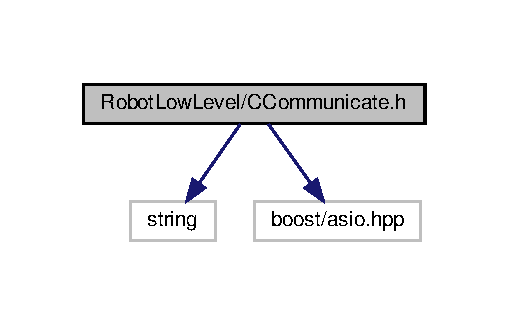
\includegraphics[width=244pt]{CCommunicate_8h__incl}
\end{center}
\end{figure}
This graph shows which files directly or indirectly include this file\+:\nopagebreak
\begin{figure}[H]
\begin{center}
\leavevmode
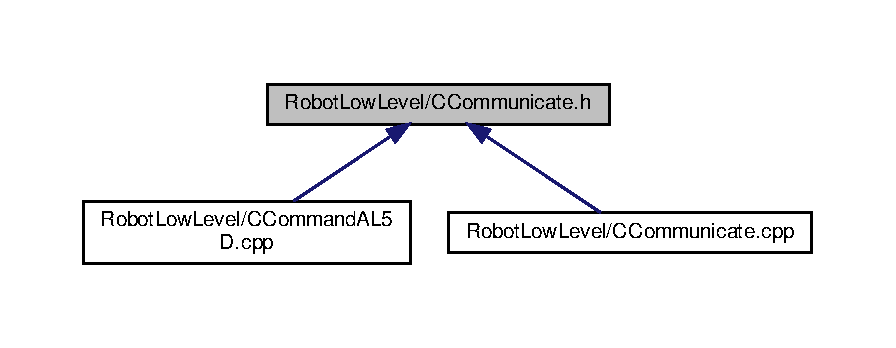
\includegraphics[width=350pt]{CCommunicate_8h__dep__incl}
\end{center}
\end{figure}
\subsection*{Classes}
\begin{DoxyCompactItemize}
\item 
class \hyperlink{classCCommunicate}{C\+Communicate}
\end{DoxyCompactItemize}


\subsection{Detailed Description}
The communicate class makes use of boost asio messaging to write messages to the robotarm through the serial output. 

\begin{DoxyAuthor}{Author}
Tim Beeren (\href{mailto:T.Beeren1@student.han.nl}{\tt T.\+Beeren1@student.\+han.\+nl}) 
\end{DoxyAuthor}
\begin{DoxyVersion}{Version}
0.\+1 
\end{DoxyVersion}
\begin{DoxyDate}{Date}
06-\/03-\/2020
\end{DoxyDate}
\begin{DoxyCopyright}{Copyright}
Copyright (c) 2020 
\end{DoxyCopyright}

\hypertarget{IExecuteCommand_8h}{}\section{Robot\+Low\+Level/\+I\+Execute\+Command.h File Reference}
\label{IExecuteCommand_8h}\index{Robot\+Low\+Level/\+I\+Execute\+Command.\+h@{Robot\+Low\+Level/\+I\+Execute\+Command.\+h}}


The Execute\+Command interfaces gives higher level drivers the ability to send instructions to the robotarm.  


{\ttfamily \#include $<$iostream$>$}\newline
{\ttfamily \#include $<$vector$>$}\newline
Include dependency graph for I\+Execute\+Command.\+h\+:\nopagebreak
\begin{figure}[H]
\begin{center}
\leavevmode
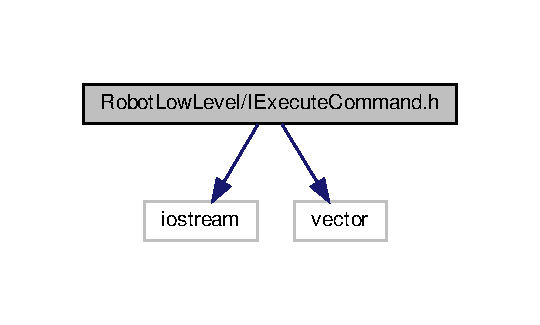
\includegraphics[width=259pt]{IExecuteCommand_8h__incl}
\end{center}
\end{figure}
This graph shows which files directly or indirectly include this file\+:\nopagebreak
\begin{figure}[H]
\begin{center}
\leavevmode
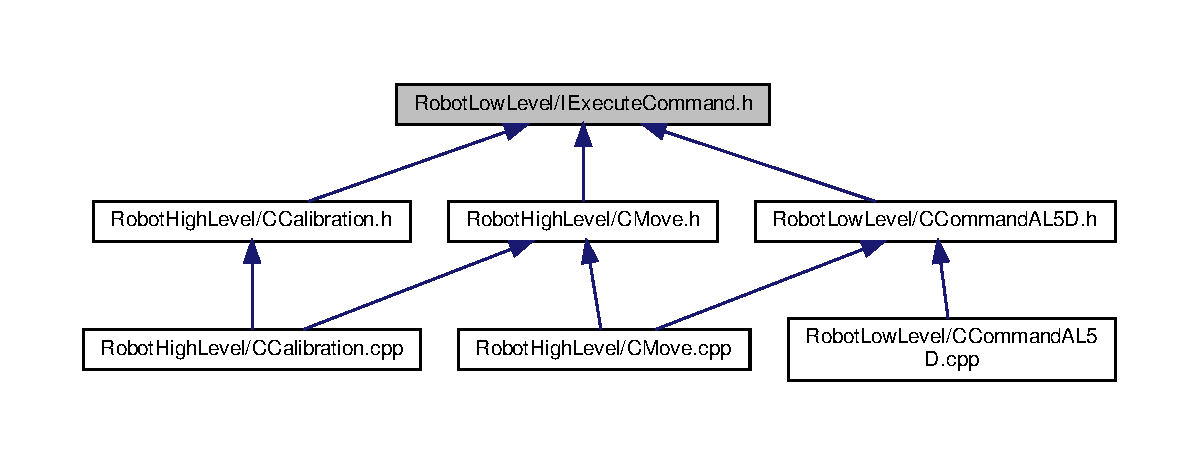
\includegraphics[width=350pt]{IExecuteCommand_8h__dep__incl}
\end{center}
\end{figure}
\subsection*{Classes}
\begin{DoxyCompactItemize}
\item 
class \hyperlink{classIExecuteCommand}{I\+Execute\+Command}
\end{DoxyCompactItemize}
\subsection*{Enumerations}
\begin{DoxyCompactItemize}
\item 
\mbox{\Hypertarget{IExecuteCommand_8h_af3a63f674d38acb98a175b1fc24bd78c}\label{IExecuteCommand_8h_af3a63f674d38acb98a175b1fc24bd78c}} 
enum {\bfseries e\+Command} \{ {\bfseries M\+O\+V\+E\+\_\+\+C\+O\+M\+M\+A\+ND} = 0, 
{\bfseries C\+A\+L\+I\+B\+R\+A\+T\+E\+\_\+\+C\+O\+M\+M\+A\+ND} = 1, 
{\bfseries S\+T\+O\+P\+\_\+\+C\+O\+M\+M\+A\+ND} = 2, 
{\bfseries U\+N\+K\+N\+O\+W\+N\+\_\+\+C\+O\+M\+M\+A\+ND} = 3
 \}
\end{DoxyCompactItemize}


\subsection{Detailed Description}
The Execute\+Command interfaces gives higher level drivers the ability to send instructions to the robotarm. 

\begin{DoxyAuthor}{Author}
Tim Beeren (\href{mailto:T.Beeren1@student.han.nl}{\tt T.\+Beeren1@student.\+han.\+nl}) 
\end{DoxyAuthor}
\begin{DoxyVersion}{Version}
0.\+1 
\end{DoxyVersion}
\begin{DoxyDate}{Date}
06-\/03-\/2020
\end{DoxyDate}
\begin{DoxyCopyright}{Copyright}
Copyright (c) 2020 
\end{DoxyCopyright}

%--- End generated contents ---

% Index
\backmatter
\newpage
\phantomsection
\clearemptydoublepage
\addcontentsline{toc}{chapter}{Index}
\printindex

\end{document}
